\chapter{{Verb phrases}}\label{sec:6}

This is the second linguistic chapter with a focus on the salient markers and characteristics of Ship English. This chapter on \isi{verb} phrases begins with the simplest realization of any \isi{verb} constituent as a single word and continues with the expansion of the \isi{verb phrase} as it incorporates \isi{tense}, modality and aspect. Subsequently, \sectref{sec:6.1}, verbs in Ship English, opens with a discussion of how the variety favors a [\isi{non-specific verb} + \isi{specifying nominal complement}] construction in which the syntactic \isi{verb} serves to introduce a \isi{nominal form} in the \isi{direct object position} which expresses the core event of the sentence.\footnote{Also know as a light verb construction.}  This sections then presents data on phrasal verbs and negation markers. The second section, 6.2 on tense, discusses present and past \isi{tense variation} and features a discussion of the potential role of the Northern Subject Rule, \footnote{The Northern Subject Rule, described by  \citet{deHaas2008} as a unique variation in verbal endings specific to Northern dialects of British English that involves variation in verbal endings according to type and position of the subject.  She explains, “Finite verbs adjacent to a pronominal subject (excepting 2SG thou and 3SG, which always take -s) take a zero ending, whereas finite verbs adjacent to a nominal (Determiner Phrase or DP) subject or not adjacent to any subject take an -s ending” (\citealt{deHaas2008}: 111).} and the manifestation of Narrative Present in performative speech in addition to the presentation of potential linguistic constraints on salient zero-inflection and the use of \isi{infinitive} forms. The third section, 6.3 on the copula and auxiliary “be”, presents data on variation in the \isi{inflectional paradigm} and discusses how the \isi{verb} “be” is used and omitted in various contexts including those with \isi{aspectual} meaning. The last section, 6.4 on auxiliaries, presents data on inflectional variation and uses of auxiliary verbs such as “have” and “do” as they are used in interrogative, indicative, and conditional modalities with details on how they express \isi{aspectual meaning}. 

\section{{Verbs in Ship English}}\label{sec:6.1}

\subsection{{The [non-specific verb + specifying nominal compliment] construction}}\label{sec:6.1.1}

As discussed in chapter 5, the data indicate that Ship English favors heavy nominalization. This section shows how verbal constructions promote this perception by relying on [\isi{non-specific verb} + \isi{specifying nominal complement}] constructions, in which  verbs retain their \isi{syntactic function}, but nominals carry more semantic load compared with prototypical “heavy” verb constructions.  For example, “the first man they gave torment to” [HCA 1/9/16] rather than “the first man they tormented”, and “[they] Spyed a Sayle and gave him chase” [HCA 1/9/13] rather than “they spied a sail and chased him”. Furthermore, this usage is found in sea shanties and so speaks to the frequency and salience of the construction in cultural forms of expression, e.g., “Give ear unto the mariners” (\isi{shanty} in \citealt{Hugill1969}: 6). Other verbs such as “use” and “offer” are used with similar \isi{syntactic function} that favor the description of the event in \isi{nominal form} as the direct objects, e.g., “he used some threatenings” [HCA 1/99/22] rather than “he threatened”, and “any one that offered any hurt or violence to Clarke he would make him suffer” [HCA 1/9/51] rather than “any one that hurt…Clarke”. The use of nominals, most frequently in the position of the \isi{direct object}, to express events means that speakers can rely on semantically less-specific verbs. This consequently means that the original direct object is demoted to another nominal position, for example an indirect object, e.g., “to have satisfaction made him” [HCA 1/99/1], “Would not return him any answer” [HCA 1/52/133], and “to make him dishoner” [HCA 1/9/8]. The \isi{pronoun} “him” in all three examples above might be expressed as the \isi{direct object} of a verbal form which is semantically specific enough to actually denote the central event of the sentence on its own, e.g., “to satisfy him”, “to answer him” and “to dishonor him”. However,  “him” is expressed as the syntactic indirect object in all three Ship English examples because the \isi{direct object position} is already occupied by the nominal forms specifying the central event of the sentence, i.e., “satisfaction”, “answer”, and “dishonor”. Similarly, in the example “the \isi{prisoner} was put commander of the small sloop” (meaning that he was given command) [HCA 1/99 New Providence 1722], the use of the semantically \isi{non-specific verb} “put” necessitates that the \isi{direct object position} be occupied by a \isi{nominal form} that specifies the actual central event of the sentence “command” which forces “the small sloop” (what is commanded) into the position of the object of the \isi{preposition} in an \isi{adverbial phrase}. In short, sailors’ preference for the [\isi{non-specific verb} + \isi{specifying nominal complement}] construction means that the sentences they used favor relatively non-specific verbs and make ample use of event nominalizations. 

The \isi{verb} “make” is the most commonly used \isi{verb} in [\isi{non-specific verb} + \isi{specifying nominal complement}] constructions in the \isi{corpus}. It often denotes that an event comes to pass or is caused to happen, and this event is subsequently expressed in \isi{nominal form} , e.g., “in order to make trade” [HCA 1/99/4], “he made a resistance with a cutlass” [HCA 1/99/9], “make information against them” [HCA 1/99/7], “Freebourne made answer” [HCA 1/9/6], and “Letts goe and make an end of the fellow” [HCA 1/9/51]. Here the events “trade”, “resist”, “inform”, and “answer” are expressed in \isi{nominal form} in the \isi{direct object} positions following the usage patterns discussed in the previous paragraph. Yet the \isi{verb} “make” is worthy of individual discussion as it not only permits a \isi{noun phrase} object, but also a \isi{prepositional phrase} indicating a direction or manner of movement, e.g., “she made away from him” [HCA 1/9/18], “the informant made to her” [HCA 1/52/124], and “this examinant made for Cape Charles” [HCA 1/9/13]. Indeed, this sense of movement may explain the \isi{idiomatic usage} in the \isi{corpus} that associates the \isi{verb} “make” with travel, transit and arrival, e.g., “we made the Island” [1045.f.3/1/16], “he made the best of his way” [HCA 1/98/254], “they made what saile they could after them” [HCA 1/53/12], “he designs to make his escape” [HCA 1/99/51], and “Make all the dispatch you can” [HCA 1/101/553]. These sample clauses with the \isi{verb} “make”, whether they are expressed with nominal or prepositional complements, all illustrate the preference for the [\isi{non-specific verb} + \isi{specifying nominal complement}] construction in Ship English and is a salient feature of the \isi{corpus}. 

\subsection{{Phrasal verbs}}\label{sec:6.1.2}

Phrasal verbs in the \isi{corpus} show a tendency to be expressed as fixed expressions, in which the verb and the particle need to be adjacent. These expressions resist the insertion of an \isi{object noun} phrase or \isi{pronoun} between the main \isi{verb} and the \isi{satellite particle}. The majority of phrasal verbs occur without separation of the verbal particle(s) and \isi{satellite particle}(s), e.g., (with emphasis added) “by \textit{breaking downe} her misson mast" [ADM 106/288/40], “[he] was presently \textit{sent for up} by the said Taylor” [HCA 1/9/39], and “when they \textit{got up} the anchor” [HCA 1/99/6]. A few examples show that it was permissible to insert a direct \isi{object noun} phrase between a \isi{verb} and a \isi{satellite particle}, for example the separation of “fetch out” in the example, “he \textit{fetch’d} the captain’s charts \textit{out}” [HCA 1/99/7]. Indeed, when the \isi{direct object} of a \isi{transitive} \isi{phrasal verb} is a \isi{pronoun}, we would anticipate it to be expressed in a position separating the \isi{verb} and the \isi{satellite particle}, e.g., “they \textit{whipped} him \textit{up} again” [HCA 1/99/7]. Yet phrasal verbs in Ship English appear to resist even this type of separation. Instead, the \isi{direct object} is more commonly expressed after the complete \isi{phrasal verb}, regardless of whether it is a \isi{noun phrase} or a \isi{pronoun}, e.g., (with phrasal verbs italicized and direct objects in bold for emphasis) “\textit{call abroad} \textbf{him}” [E134/34Chas2/Mich36], “\textit{took away} out of his packett \textbf{his} \textbf{Sealed} \textbf{ring}” [HCA 1/9/18], and “they \textit{let go} \textbf{her} \textbf{anchor}” [HCA 1/52/2]. Thus, although phrasal verbs permitted separation of the \isi{verb} and the \isi{satellite particle}, it was common to keep both or all parts of the \isi{phrasal verb} together without separating them with either a nominal or pronominal \isi{direct object}. 

\subsection{{Negation}}\label{sec:6.1.3}

Negation can be marked in a variety of ways in Ship English, the most common of which was the use of the negative particle “not” after a \isi{finite verb}.\footnote{The most common pre-verbal usage of the negating marker “not” occurred in phrases headed with “being”, e.g., “he did not Duty \textit{not being well}” [HCA 1/99/108] and “the \isi{merchant} ship \textit{not being gon} into York river” [CO 5/1411/702].} Modern day speakers of English are accustomed to the particle “not” used with  “be”  used as an auxiliary verb, and this type of modern-\isi{standard usage} was evident in the \isi{corpus} (all examples emphasized), e.g., “Our Ankor \textit{was not} no sounder” [T/70/1215], “the country and his colonies \textit{was not} under his command” [CO 5/1411/101], and “the Prisoner was not only never on Board” [HCA 1/99/156]. Standard \isi{modern usage} also requires “do-support” in the negation of verbs expressed in the \isi{present tense} \isi{indicative mood}, e.g., “he \textit{does not} / \textit{doesn’t} work”, and this type of \isi{standard usage} was also evident in the \isi{corpus}, e.g., “he \textit{did not hear} it” [HCA 1/99/5], “The English \textit{did not row}” [HCA 1/13/96], “he \textit{did nott thinks} itt convenientt” [ADM 52/2/3], and “Porter complained that they \textit{did not work}” [HCA 1/99/8]. The verb “do” is also used as an auxiliary with indicative verbs despite the fact that the conjugation of the auxiliary, particularly with \isi{third person singular} subjects, does not always align with modern-day \isi{standard usage}, e.g., “Capt Rigby \textit{doe not} nor shall \textit{carry off} this land any Persons” [HCA 1/9/7], “Captain Sharp \textit{don’t forget} to Speak for us” [HCA 1/99/30], “he \textit{don’t know} that the \isi{prisoner} had any money” [HCA 1/99/10], and “[he] \textit{do’s not know} what ship” [HCA 1/99/99].\footnote{The use of “doth” in negation is rare in the \isi{corpus} and mostly seems to derive from the speech acts of judicial representatives in court records and not the sailors themselves, e.g., “he doth not know of any corespond[ance]” [HCA 1/14/140], “Doth not know the ships name” [HCA 1/14/140], and “whose name he doth not remember” [HCA 1/14/203].}  However, this type of negation using “do support” and the “not” marker for simple \isi{verb} phrases in the negated \isi{indicative mood} had a low frequency in the \isi{corpus} and may only reflect recent changes in the direction of Early Modern English. Much more salient was the use of the particle “not” immediately after the \isi{verb} and without any auxiliary marker. Examples of this type of negation appear in logbooks, e.g., “wee \textit{weighd nott}” [ADM 52/2/6], and “But [we] \textit{found not} A man in har [i.e., her]” [T/70/1215]; in journals, e.g., “I \textit{hope not} so” [445f.1/26], and “I \textit{got not} in till the next Day” [1045.f.3/1/22]; and in private correspondence, e.g., “they \textit{had not} those termes” [CO 5/1411/39], and “I \textit{doubt not}” [BL/74/816/m/11/36/1]. Yet, it was most common in witness testimony, e.g., “he \textit{intended not} to sell the said rope” [HCA 1/101/224], “She \textit{remembers not}” [HCA 1/9/51], “He \textit{cared not} what the master did” [HCA 1/9/139], “I sent for him aboard but hee \textit{came not}” [HCA 1/9/4], and “he \textit{had not} opportunity of getting away” [HCA 1/99/165]. This type of negation was even more pronounced with the \isi{verb} “know”, which showed up in negated statements repeatedly in the \isi{corpus} in both past and \isi{present tense}, e.g., “he \textit{knew not} the design of the others” [HCA 1/99/5], “he \textit{knew not} when he would return” [HCA 1/14/151], “he \textit{knew not} but that he might prosecute him” [HCA 1/52/46], “He \textit{knowes not} of any Nutmeggs or Cloves” [HCA 1/12/78], “whose names I \textit{know not}” [BL/74/816/m/11/36/3], “I \textit{know not} of any methods” [CO 5/1411/655], and “He \textit{knows not} nor ever heard” [HCA 1/9/51]. However, negation with the “not” marker was versatile and permitted syntactic variation; for instance, it occurs in a position separated from the \isi{verb} by a pronominal \isi{direct object} (emphasized in bold), e.g., “wee \textit{saw}\textbf{ }\textbf{him} \textit{not}” [HCA 1/12/2], “yet [we] \textit{made} \textbf{him} \textit{not} Bear for our company” [T/70/1216/13], “he \textit{has} \textbf{it} \textit{not} for himself” [HCA 1/99/51], and “They \textit{found} \textbf{it} \textit{not} safe to hazard” [ADM 51/4322/4]. Indeed, “not” was the most versatile and the most common \isi{negation marker} in the \isi{corpus}, and based on a sample of 204 items (see \figref{fig:key:6.1}), accounts for more than half of all negated \isi{verb} phrases. In sum, although the salient “not” \isi{negation marker} was used in a manner comparable to modern-day usage of the verb “be” and with “do-support”, it was more frequent in a variant \isi{post-verbal position} without any auxiliary marker. \footnote{Negation using “not” with auxiliaries of conditional modality also feature in the \isi{corpus}, but are discussed in \sectref{sec:6.4.3} Modal Auxiliaries.} 

  
\begin{figure}
\footnotesize
\begin{minipage}[c]{.28\textwidth}%
\begin{tabular}{ll}
\lsptoprule
Marker & No.\\
\midrule 
Not & 104\\
Never&42\\
No&25\\
Nor& 17\\
Nothing&8\\
Neither&3\\
No one&3\\
Prefix <un> & 2\\
\midrule
& 204\\
\lspbottomrule
\end{tabular}\end{minipage}%
\begin{minipage}[c]{.72\textwidth}%
\begin{tikzpicture}\footnotesize
%   [
%       pie chart,
%       slice type={Not}{lsDarkBlue},
%       slice type={Never}{lsMidBlue},
%       slice type={No}{lsMidDarkBlue},
%       slice type={Nor}{lsLightBlue},
%       slice type={Nothing}{lsDarkGreenTwo},
%       slice type={Neither}{lsRichGreen},
%       slice type={Noone}{lsLightGreen},
%       slice type={un}{lsMidGreen},
%       scale=4
%   ]
%   \pie[text=pin,radius=2,color={lsMidBlue,lsLightGreen,lsMidGreen,lsLightBlue},/pgf/Minimum Angle=8,]{49/Adjective,32/Noun,18/Adverb,1/Infinitive (1\%)}  

  \pie[text=pin,radius=3,sum=auto,color={lsDarkBlue,lsMidBlue,lsMidDarkBlue,lsLightBlue,lsDarkGreenTwo,lsRichGreen,lsLightGreen,lsMidGreen},pgf/Minimum Angle=8]{104/Not,42/Never,25/No,17/Nor,8/Nothing,3/Neither (3),3/No one (3),2/Prefix \textit{un-} (2)}
% 	21/Never,
% 	12/No,
% 	8/Nor,
% 	4/Nothing,
% 	2/Neither,
% 	1/Noone,
% 	1/un}  
%   \legend[shift={(1.5cm,17mm)}]{{Not (104)}/Not, 
% 			    {Never (42)}/Never,
% 			    {No (25)}/No,
% 			    {Nor (17) }/Nor,
% 			    {Nothing (8)}/Nothing,
% 			    {Neither (3)}/Neither,
% 			    {No one (3)}/Noone,
% 			    {Prefix \textit{un-} (2)}/un}
\end{tikzpicture}\end{minipage} 
\caption{\label{fig:key:6.1}: Distribution of negation markers used in a sample of 204 verb phrases\\
{\tiny Sources: 1045.f.3/1, 445f.1, AC WO 16–16/8–16, ADM 51/4322, 3983, 3954, ADM 52/1, 2, BL/74/816/m/11/36, CO 5/1411, DDB6 8/4, HCA 1/9, HCA 1/11,12,13,14, HCA 1/52, HCA 1/98, 99, 101, Palmer (1986]. SP 42/6, T/70/1215.}
}
% \todo[inline]{fix legend}
\end{figure}


The second most common \isi{negation marker} in the sample was the word “never” which was used both to mark categorical denial over time (as in standard \isi{modern usage}) and to mark the negation of a simple \isi{verb} form with no \isi{aspectual meaning}. Given that the term “never” derives etymologically from the negative particle “ne” (meaning “no”) and the \isi{adverb} “ever”, the most transparent meaning of the negative marker is one associated with a \isi{durative aspect} and the most logical context is with a situation of zero-possibility with a cumulative quantification over time, i.e., something that has categorically not happened up to and including the present moment. This meaning is evident in the \isi{corpus} (all marked for emphasis), e.g., “he did not hear it Read, nor \textit{never} heard that it was read” [HCA 1/99/5], “he had \textit{never} been arrested of any ill action” [HCA 1/99/8], “was \textit{never} till now taken” [HCA 1/13/95], “was \textit{never} before seen by him” [HCA 1/13/92], and “\textit{Never} had any acquaintance or discourse with nor ever saw the said Prock or Richard [...] before” [HCA 1/52/133]. However, less than a quarter of the “never” negation markers in the sample, only 10 of the 42 items sampled, had the meaning “no(t) ever”, see \figref{fig:key:6.1}.

The majority of examples of “never” were used with specific durations of time or to negate indicative \isi{past tense} situations. The marker “never” used to negate specific durations of time and that frequently occurs with adverbs such as “(un)til” or “since” is comparable to negation in \isi{perfect aspect} or with \isi{preterit} verbs in modern standard English. For example, “he \textit{never} was at attacking any Ship, Since he has been among them” [HCA 1/99/80] is comparable to \isi{perfect aspect} negation in modern-day usage, i.e., “he \textit{had not attacked} any ship since he had been among them”. In contrast, “he \textit{never} knew the prisoners till taken in the boat” [HCA 1/99 \isi{Bahama} Islands 1722] is comparable to \isi{preterit} negation in modern-day usage, i.e., “he \textit{didn't know} the prisoners until taken in the boat”. Even more common than this, however, was the use of “never” to negate events with little or no evidence of \isi{durative aspect}, e.g., “[on] July the 16th 1720, [he] owned he helped travessing a Gun but \textit{never} fired” [HCA 1/99/78], “he knew very well he had \textit{never} signed the Articles” [HCA 1/99/62], “he \textit{never} see him Sober Scarce” [HCA 1/99/44], and "Shows [shoes], stocking, which \textit{never} cost about [...] shillings” [SP 42/6]. Some examples of this type of indicative \isi{past tense} negation are only evident in light of the context of the utterance, e.g. the defendant who claims he “did \textit{never} see any letter” [HCA 1/98/255] is clearly referring to a specific letter at a specific time and not “any” letter at any previous time in his life (as would be implied by the use of “never” meaning “not” + “ever”). Similarly, when John Barefoote, Yeoman of the powder room of the \textit{Antelope} during April of 1663, testifies that he “\textit{never} had any discourse with Nathaniel Paintor Armourer in the \textit{Anthelope} nor with any other person in the said shipps Gunroome” [HCA 1/9/63] he is most likely referring to a specific conversation on a specific day (and hence, \isi{preterit} negation) rather than the idea that he “never” spoke with the armorer of the vessel nor any other person in the gunroom — an unlikely claim given that his job was to store and manage the gunpowder. Thus, whether it is evident from the linguistic context of the clause itself or the wider socio-historical context of the \isi{speech act}, the majority of negated statements using “never” appear to denote indicative past negation and not any kind of \isi{durative aspect} that we might associate with a \isi{lexeme} that derives from the negative particle “ne” and the \isi{adverb} “ever”.\footnote{It is worth noting that this past indicative use of the adverb “never” without \isi{durative aspect} is still found (in addition to other variant uses with varying degrees of \isi{aspectual} meaning) in modern-day non-standard English dialects (see \citealt{LucasWillis2012}).}  

The third and fourth most common \isi{negation marker}s in the sample were the words “no” and the conjunction “nor”, which sampled at 12 and 8 percent of the total number of examples, respectively (see \figref{fig:key:6.1}). The negative marker “no” was most typically used in a prenominal position before a direct object or object compliment and took the function of a zero-marking determiner, e.g., “wee having noe boate” [HCA 1/12/2], “we found noe ground with our hand line” [ADM 52/1/7], “he thought himself no robber” [HCA 1/99/23], “Being able to get no imploy” [HCA 1/13/97], and “He knew of no offense that he had done therefore would ask him no pardon” [HCA 1/52/14]. This method of negation functions in accordance with the previously discussed tendency in Ship English to favor nominalization using light verbs, e.g., “Wee tooke no harme” [ADM 51/3983/1], “The Governour was a board of us but made no stay” [ADM 52/1/8], “but knows of no Sharing they made” [HCA 1/99 New Providence 1722], and “no vessell comeing that year could make noe prize” [HCA 1/98/262]. The negative marker “nor”,  instead of being used in a pre-nominal position after an inflected \isi{verb}, often preceded a non-\isi{finite verb}, e.g., “he nor seeing them come out nor dealing with the master” [T 70/1/10] and “nor being neither this Deponent” [HCA 1/14/51]. However, the more customary use of “nor” as a negating conjunction frequently occurs in the \isi{corpus} and often functions to conjoin constituents that already have negation. Such \isi{negative concord} was a salient feature of sailors’ speech that manifests itself in popular songs about life at sea, such as the seventeenth-century song “Another of Seafarers” that includes the line “Nor have no room” (cited in \citealt{Palmer1986}: 6). The simplest example of negative concord in the \isi{corpus} is the word “nor” used to conjoin two negated \isi{verb} phrases, e.g., “He knows not \textit{nor} ever heard” [HCA 1/9/51] and “he …did \textit{not} bye them \textit{nor} had \textit{not} any conferences” [HCA 1/101/221]. In addition to concordant markers of negation occurring in the same phrase, strings of negated clauses are also common in the \isi{corpus}, for instance, the witness statement “But knows \textit{not} what it was, for he did \textit{not} hear it Read, \textit{nor never} heard that it was read, \textit{nor} knows \textit{not} how the Vessell was fitted out” [HCA 1/99/5] includes 6 negation markers, “not” (used three times both in a post verbal context and with “do support”), “nor” (twice), and “never” (once). The conjunction “nor” functions to join three negated clauses, firstly, “for he did \textit{not} hear it Read”, secondly, “\textit{never} heard that it was read”, and lastly “\textit{nor} knows \textit{not} how the Vessell was fitted out” and all of these are prefaced by another negated clause “But knows \textit{not} what it was” making a string of four negated clauses. A few times, the negative particle “nor” occurs as part of a correlative conjunction with the word “neither”, e.g., “he \textit{neythor} aske any price of the said Sherman for the said goods \textit{nor} the said Sherman never asked him if he would sell them or not” [HCA 1/101/224]. Yet, even in these few instances, the clauses that are conjoined often include \isi{negative concord} within the conjoined structure, such as in the example, “\textit{nor} the said Sherman \textit{never} asked him if he would sell them or \textit{not}.” This type of \isi{negative concord} may have been a feature of Ship English, but it was not distinctive from other varieties of English. The phenomena of \isi{negative concord} in non-standard varieties of English is widespread  around the modern-day Atlantic (\citealt{vanderAuwera2016}), and (\citealt{KortmannLunkenheimer2013}) attest to  80\% \isi{negative concord} among global varieties of English . Thus, \isi{negative concord}, specifically using “no” in a prenominal position and joining negated phrases or clauses with the conjunction “nor”, is a salient feature of Ship English, but this is not surprising given its occurrence in Old English and its persistence throughout history up to the modern day in variant negation systems throughout the Anglophone world.  

\section{{Tense}}\label{sec:6.2}

\subsection{{Present tense variation} }\label{sec:6.2.1}

Logbooks, letters and depositions alike show variation in inflection patterns for \isi{present tense} \isi{indicative modality}, specifically an absence of inflection with \isi{singular third person} subjects. The following examples show \isi{uninflected} finite verbs (emphasized by italics) with \isi{singular third person} \isi{noun} phrases (emphasized in bold) “\textbf{moderate} \textbf{weather} \textit{blow} fresh” [ADM 52/2/3], “\textbf{Our} \textbf{boat} \textit{goe} in to Black Slakes” [ADM 52/2/9], “\textbf{all} \textbf{shipping} that \textit{come}” [BL/Egerton 2395/0007], and “\textbf{the} \textbf{boat} \textit{want} for wood” [CO 5/1411/712]. One specific \isi{witness deposition} taken in Grand \isi{Bahama} Island and dated 1722 shows inflection as a superscript particle (see \figref{fig:key:6.2}) suggesting that the original statement may not have included the inflection but it was added at a later stage in the \isi{court clerk}’s revisions. In addition to the examples of verbs used with \isi{singular third person} \isi{noun} phrases, there is also evidence of zero inflection with \isi{singular third person} pronouns, e.g., “\textbf{whoever} \textit{see} one first” [HCA 1/99/143], “He swore that \textbf{he} \textit{know} no negroes” [T 70/1/5], “\textbf{He} \textit{know} of no commission” [HCA 1/9/10], “\textbf{he} \textit{know} not” [HCA 1/101/219], and “\textbf{He} well \textit{know} Joseph Passof” [HCA 1/14/150]. Examples appear to connect the zero inflection with negation and specifically the \isi{verb} “know”, suggesting that this variation may be conditioned by linguistic constraints or favored specific lexemes in idiomatic phrases, however, the potential role of the Northern Subject Rule might also affect the selection of zero inflection with \isi{third person} pronominal subjects (see  \citealt{deHaas2008}). 

 
\begin{figure} 
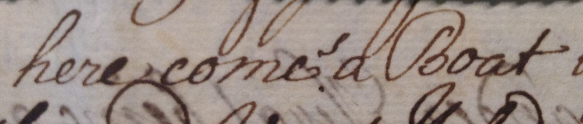
\includegraphics[width=\textwidth]{figures/delgado-img16.png}

\caption{\label{fig:key:6.2} Excerpt from a deposition showing superscript inflection with a third person singular noun phrase in present tense indicative modality [HCA 1/99 Bahama {Islands 1722}]}
\end{figure}


The Northern Subject Rule may also account for examples of atypical inflection with \isi{plural} \isi{third person} subjects and when the \isi{verb} is not adjacent to a subject. In the \isi{corpus}, some \isi{plural} \isi{third person} subjects that are expressed as \isi{noun} phrases (emphasized in bold) take an inflected \isi{verb} (emphasized in italics), e.g., “\textbf{the} \textbf{barracks} \textit{tooks} fire” [SP 42/6], “\textbf{severall} \textbf{papers} which \textit{comes} herewith” [SP 42/6], and “\textbf{which} \textbf{accts} plainly \textit{demonstrates} the tricks” [SP 42/6]. The last two examples show the inflected \isi{verb} in a position that is not immediately adjacent to the \isi{noun phrase} subject, and perhaps this was a conditioning factor in the use of inflection with \isi{third person} subjects. Yet, whether it was due to the Northern Subject Rule, or another conditioning factor, the atypical inflection with \isi{plural} \isi{third person} subjects in Ship English — particularly when the \isi{verb} is not adjacent to a subject — was salient enough to be recorded in \isi{seventeenth century} sea-songs, e.g., “They cried \textbf{Englishmen} \textit{comes}” (from “A joyful new Ballad” cited in \citealt{Palmer1986}: 16), and “\textbf{Brave} \textbf{sailors} that \textit{sails} on the main” (from “Sailors for my Money” cited in \citealt{Palmer1986}: 31). Thus, although the constraints of the variation within inflectional paradigms are not entirely clear, sailors of the period were known to inflect verbs in ways that did not follow conventional contemporary standards. 

In addition to variation in \isi{present tense} inflection, there is also evidence of \isi{present tense} use in past contexts. Logbook entries clearly marked for past context make use of verbs inflected for the present indicative \isi{tense}, e.g., (with italic emphasis), “Last night the wind \textit{proves} Westerly” [ADM 52/2/9]. Witness depositions feature the use of \isi{present tense} more heavily despite the fact that the statements are marked for past context by the nature of their narrative content and also by the use of other \isi{preterit} verbs (emphasized in bold), e.g., “Then the Captain \textit{goes} upon the Half-Deck again, and \textbf{call’d} to his Man” [445f.1/23], and “the \isi{mariner} \textbf{Lay} and there \textit{talkes} with the men” [HCA 1/101/217]. Indeed, the use of inflected \isi{present tense} in past contexts in alteration with \isi{preterit} forms may be a manifestation of the narrative function of witness statements. Fleischman explains, “the NP [Narrative Present] is a spontaneous use of the PR [\isi{present tense}] that occurs consistently in \textit{alternation} with tenses of the P [past] and is linked to a performative mode of \textit{oral} storytelling” (1990: 258, author’s italics). Witness statements are certainly a modality of oral storytelling and in this context, alternation from past to present forms may have helped sailors bring immediacy — and thereby credibility — to their performances in court. The same use of Narrative Present \isi{tense} features in journal writing, e.g., Angelo and De Carli’s published work, “A Curious and Exact Account of a Voyage to Congo in the Years of 1666 and 1667” that narrates events alternating between \isi{present tense} forms (in italics) and \isi{past tense} forms (in bold):

\begin{quotation}
In a little time \textit{comes} the Lieutenant, and \textit{says} to one of them, Go down to thy Quarters; his answer \textbf{was}, I \textit{can} Fight no more; The which \textbf{was} what he looked for; for he \textbf{was} our greatest Enemy. Then he \textit{goes} to the captain, and \textit{makes} the worst of it, saying, Yonder the Quakers be altogether, and I \textit{do not know} but they \textit{will} Mutiny, and one \textit{says} he \textit{cannot} Fight; then he \textbf{ask’d} his name and \textbf{came} down. [445f.1/23]
\end{quotation}

Although the use of the \isi{present tense} is understandable in the representations of direct speech in this excerpt, narrative phrases also use \isi{present tense} to provide immediacy for the reader. So, although we might anticipate that the oral performance of witness testimony be more likely to show evidence of the Narrative Present, examples suggest that sailors also alternated between past and present in logbooks and journals, potentially reflecting their oral and performative culture (discussed in Chapter 4, Section 4.2.6 on shared ideologies and leisure activities). 

\subsection{{Past tense variation} }\label{sec:6.2.2}

Variation in \isi{past tense marking} was one of the most salient features in the \isi{corpus}. There are many examples of regular inflection with weak (i.e., regular) \isi{verb} stems, (emphasized by italics) e.g., “we \textit{stopped} our ship” [ADM 52/2/5], “he \textit{answered} that he does not know” [HCA 1/13/94], and “he came afterwards \&  \textit{robbed} her” [HCA 1/99/41]. Even with non-standard orthography, many examples of verbs imply pronunciation of the regular \isi{past tense} suffix <ed>, e.g., “[he] \textit{call’d} to his Man” [445f.1/23], “wee \textit{stopt} the Ebb all the flett \textit{Ankerd}” [ADM 52/2/1], “wee \textit{waid} [weighed] Anker” [ADM 52/2/1], “Both his pistolls \textit{mist} [missed] fire and did not go off” [HCA 1/52/137], and “\textit{kist} [kissed]… \textit{tript} [tripped]” [HCA 1/99/11].\footnote{In addition to these accepted regular forms of \isi{preterit} weak verbs, the use of “-th” inflections were also acceptable in the Early Modern English period, e.g., “who \textit{giveth} him dayly wages” [HCA 1/101/219] and “[he] \textit{saith} hee did” [HCA 1/9/3], although they were not a dominant form in the \isi{corpus}.} However, there were also many examples of weak finite verbs that were not inflected in a regular \isi{preterit} form despite being contextualized in the \isi{past tense} (by virtue of their narrative content and/or the past inflections of adjacent \isi{verb} phrases). Excerpts from depositions illustrate this phenomenon (emphasized by italics), e.g., “he \textit{fetch} some wine and \& beer” [CO 5/1411/47], “He \textit{hoyst} sayle \& went from that place” [HCA 1/52/41], “The Carpenter… came up, and \textit{answer} to the captaine” [HCA 1/52/41], and “[the men] \textit{board} and \textit{board} in which severall men were killed” [HCA 1/53/3]. Note that in the last three examples the unmarked forms are used in collocation with the \isi{preterit} forms of strong verbs, “went”, “came”, and “were”, respectively, which not only mark the past context of the excerpt but also show that unmarked forms were not universal in individual speech acts or for individual speakers. Similarly, excerpts from logbooks also include frequent \isi{uninflected} weak verbs in the \isi{past tense}, e.g., from the logbook of the \textit{Pideaux:} “this morning we \textit{lift} him again” and “he \textit{lift} the vessel” [HCA 1/99/53] and from the logbook of the Albemarle: “at 9 at night wee \textit{anker} in 30 fathom water”, “in the afternoon we \textit{fetch} 3 boat Loads of Ballast”, “at night we weighed \& \textit{fill up} the boy”, and “We \textit{Bury} overboard another Wounded” [ADM 52/2/1,6,8,9]. Although a number of the examples from logbooks follow prepositional phrases marking time, this is not considered to be a linguistic constraint of unmarked \isi{preterit} forms as there are also many examples of weak verbs with regular <ed> suffixes in this context. In short, it appears that Ship English permits \isi{free variation} between regular weak \isi{preterit} forms and unmarked \isi{preterit} forms, and this can occur across a range of registers, modalities, and linguistic contexts. 

Strong verbs (i.e., irregular verbs) presented the most variation in \isi{past tense marking}. There are many examples of strong \isi{preterit} forms in the \isi{corpus}, e.g., (with italic emphasis) “and [I] \textit{spoke} with him” [CO 5/1411/700], “They \textit{took} and plundered and \textit{took out} some rice \& sugar” [HCA 1/52/75], and “he \textit{saw} the \isi{prisoner} have a Sword” [HCA 1/99/72]. Yet, numerous examples also attest to variant methods of marking the \isi{preterit}. In some excerpts, past participles are used as \isi{preterit} forms of strong verbs, e.g., “he \textit{seen} him cut her cable” [HCA 1/99/73], “he \textit{seen} him go on Board” [HCA 1/99/96], and “[we] \textit{Rid} all night” [ADM 52/2/6].\footnote{According to \citet[95]{Blake2002} the \isi{preterit} and \isi{past tense} forms were encroaching into each other’s syntactic space in the Early Modern English period and so this type of variation may have been common at the time. Furthermore, this usage remains common in some modern non-standard varieties (\citealt{Cheshire1994}: 125).} Other excerpts show alternative irregular \isi{preterit} forms, e.g., “I \textit{writ} from Leverpoole” [445f.1/46], “I am informed of a letter you \textit{writ}” [HCA 1/98/66], and “we \textit{kam} to Anankor" [DDB6 8/4].\footnote{The \isi{preterit} in the example “we kam to Anankor" [DDB6 8/4], is somewhat problematic and depends on the speaker’s realization of the orthographic ‘a’ which appears to be [{ӕ] but could just have likely been realized as the diphthong [{ɪ}] or another allophonic variant acceptable in contemporary usage.} } The most common inflected variant however was a regularized form of a strong \isi{preterit} that was marked with a regular <ed> suffix, e.g., “He should not be \textit{hurted}” [HCA 1/99/9], “[I] \textit{quitted}” [HCA 1/99/12], “he \textit{waked}” [HCA 1/99/4], “she went out and \textit{catched} the Swallow” [HCA 1/99/150], and “[he] \textit{threw’d} the Dept. against the Ladder” [HCA 1/99/152]. The last example is particularly interesting as it marks \isi{tense} twice, once in the form of the anticipated strong \isi{preterit} form “threw” and again with the regular inflection “-ed” common to weak verbs. This example appears to corroborate the double \isi{tense marking} that Bailey and Ross found in logbook entries: “we \textit{bored} the yards” (1688: Sloane 3671) and “we \textit{tookt} in the Virgins Prises” [ADM 51/4298 1692] (cited in \citealt{BaileyRoss1988}: 204). It also potentially corresponds with the type of concordant \isi{past tense marking} in examples using an \isi{auxiliary verb}, e.g., “\textit{Did found} Robert Clarke” [HCA 1/9/51] that marks \isi{past tense} once in the \isi{auxiliary verb} “did” and again in the strong \isi{preterit} “found”. There were no discernable linguistic constraints that governed selection of \isi{past tense} realization, and some documents written in the same hand show \isi{free variation} in similar linguistic contexts, e.g., the journal of \isi{mariner} and \isi{merchant} Bryan Blundell (1687–1754) that includes the phrase “[the wind] \textit{blowed} very hard” and also “the wind \textit{blu} very hard” [DDB6 8/4] showing examples of the regularized \isi{past tense} form and the irregular form by the same author. 

Just like their weak counterparts, strong verbs also frequently occur without any \isi{past tense marking}, and this was the most common variant realization in the \isi{corpus} for this type of \isi{verb}. Strong verbs in witness testimony narrating past events frequently show zero marking, (emphasized by italics), e.g., “hee well \textit{know}” [HCA 1/52/1], “\textit{strike} him severall bloes about the head” [HCA 1/11/74], “He left one \&  \textit{Bring} one to us” [ADM 52/2/9], “he \textit{say} that” [HCA 1/98/24], and “he was a Brisk Fellow [...] and \textit{tell} Roberts” [HCA 1/99/132]. Strong verbs in logbook entries relating to recent events in the \isi{past tense} also show frequent zero marking, e.g., “Longboat in a Violent Gust \textit{break}” [ADM 51/3954], “The wind \textit{blow} fresh” [ADM 51/4322/1], “we \textit{gett} 32 punsh [punch] \& 31 butt ashore” [ADM 52/1/8], “wee \textit{give} Our ship” [ADM 51/3797/1]. Although the frequency of zero-marked \isi{preterit} strong verbs is significant for a range of verbs both in logbooks and witness depositions, there were some trends that suggest a higher usage with specific verbs. The \isi{verb} “see” was sampled with zero \isi{past tense marking} 21 times (significantly more than any other \isi{verb}) throughout the \isi{corpus}, e.g., “I \textit{see} him put it under his left arm” [HCA 1/99/7], “he \textit{See} him go over the Side” [HCA 1/99/147], “he \textit{see} him cruelly beat to make him go” [HCA 1/99/147], “hee \textit{see} George Freebound” [HCA 1/9/3], and “In Hasting Bay wee \textit{see} Severall French Shipps” [ADM 52/3/7]. Four counts of zero marking with negation imply a possible condition, e.g., “he never \textit{see} them any more” [HCA 1/99/110], “never \textit{see} him in Arms” [HCA 1/99/133], “never \textit{see} any Letter” [HCA 1/98/20], and “Gott about the mast but \textit{see} nothing but three small Topsails” [ADM 52/3/7]. However, there is little evidence that this specific \isi{verb} is conditioned by any specific factors that select zero \isi{preterit} marking and the strong \isi{preterit} form is equally represented in the \isi{corpus} (including in phrases with negation) e.g., “had never saw a Prize taken” [HCA 1/99/8], “wee saw him not” [HCA 1/12/2], “At two yesterday [...] \textit{saw} our fleat” [ADM 52/1/1], “he \textit{saw} the \isi{prisoner} have a Sword” [HCA 1/99/72], and “he run away when he saw twas the Kings Ship” [HCA 1/99/96]. Thus, the lexical item itself rather than the linguistic context of its use appears to select a preference for zero marking, although zero marking occurs with a range of verbs and is not restricted to specific lexical items like the \isi{verb} “see”.

The \isi{verb} “run” was the second most heavily occurring strong \isi{verb} with an unmarked \isi{preterit} form, sampled 18 times in the \isi{corpus}. Every one of the 18 examples occur in the context of a \isi{phrasal verb} (emphasized in italics) e.g., “he \textit{run up} the shrouds” [HCA 1/99/9], “\textit{Run out} to the buoy” [ADM 52/2/5], “they \textit{run} her \textit{on} ground” [HCA 1/99/10], and “he Saw the Kings Colours he \textit{run down}” [HCA 1/99/78]. As in the last example, many of these unmarked phrasal verbs occur in contexts where other strong \isi{preterit} forms and weak \isi{preterit} forms are explicitly marked for \isi{past tense} (marked in bold), e.g., “when he \textbf{Saw} the Kings Colours he \textit{run down}, \textbf{Confessed} he had been on Board” [HCA 1/99/78], and “we \textbf{shote} his maine yard Down but he \textit{run over} the officer and \textit{run up} Poldard bay [...] where he \textbf{durst} not follow” [ADM 52/1/1]. The \isi{satellite particle} “away” used with the \isi{verb} “run” appears to favor zero \isi{past tense marking} more than any other \isi{satellite particle}. This is evidenced by the fact that “run away” composes more than half of the recorded samples using the \isi{verb} stem “run” (10 of the 18 samples),\footnote{The high frequency of “run away” may, in part, be explained by the nature of witness testimony coupled with the number of court cases related to sailors deserting their vessel.} e.g., “John Hardin who \textit{run} away” [SP 42/6], “one of them who run away with the sloop” [HCA 1/99 \isi{Bahama} Islands 1722], “Kenyou \textit{run away} crying what have you done” [HCA 1/99/7], “he \textit{run away} when he saw twas the Kings Ship” [HCA 1/99/96], and “Some men that \textit{Run away}” [HCA 1/13/100]. Yet “run” (with whatever \isi{satellite particle} it takes) is not the only \isi{verb} stem in a \isi{phrasal verb} that is represented with zero marking in the \isi{corpus}. Various \isi{uninflected} verbs with a range of satellite particles also select zero marking, e.g., “We \textit{goe away} Before” [ADM 52/2/9], “The Cable \textit{give waye}” [ADM 51/3797/1], “His Company aforesaid and \textit{take away} his said Vesell” [HCA 1/52/133], “At two yesterday [...] saw our fleat then we \textit{hall in}” [ADM 52/1/1], “A saile \textit{stand out} of the Ba [bay]” [ADM 52/2/9], “We soon \textit{come up with} her” [ADM 52/2/9], “Watts \textit{take off}” [HCA 1/99/145], and “I \textit{come to} an Anchor” [1045.f.3/1/16]. In short, although “run”, specifically used with the \isi{satellite particle} “away”, was the most salient example of unmarked strong \isi{preterit} forms in the \isi{corpus} when expressed as a \isi{phrasal verb}, evidence indicates that Ship English permits zero marking in any \isi{phrasal verb} composition, although certain lexemes might favor zero marking in \isi{idiomatic usage}. 

As discussed in the previous paragraphs, \isi{past tense} variant forms may be conditioned by certain lexemes such as “see” and “run” or they may be conditioned by verbs used in \isi{phrasal verb} constituents, yet overall there is no convincing evidence that linguistic or socio-linguistic factors play a role in past \isi{tense variation}. Instead, variant forms occur in the same linguistic contexts, in the same documents, and in the same handwriting across a range of documents with varying levels of formality and stylistic expectations. For example, one \isi{witness deposition} includes the statement, “They \textbf{took} and \textbf{plundered} and took out some rice \& sugar and some rigging and then \textit{sink} her” [HCA 1/52/75] in which an unmarked \isi{preterit} “sink” occurs in a coordinated clause structure with the standard inflected weak \isi{verb} in \isi{past tense} “plundered” and also the standard form of the strong \isi{verb} \isi{preterit} “took”. Logbooks also show examples of zero marked \isi{preterit} forms in coordinated clauses with standard forms of strong verbs, e.g., “severall of the fleet \textit{break} their Cables \& we \textbf{lost} our Long boat” [ADM 52/2/6], and “every one \textbf{came} and \textit{eat} and \textbf{drank} with him” [HCA 1/99/59]. Other logbooks show the same \isi{verb} occurring in standard and \isi{preterit} forms in a single \isi{speech act}, e.g., the \isi{verb} forms “gett” and “gott” in the excerpt, “We \textit{gett} Anchor aboard [...] we \textit{see} severall ships a stern which \textbf{Came} into our fleet … severall of the fleet \textbf{made} Sayle and \textbf{gott} into [...] harbor” [ADM 52/3/7]. A longer excerpt from a single witness statement taken at the Rhode Island and Providence Plantation on 9 September {1725} shows similar variation among standard and zero-marked forms of strong verbs by one speaker:

\begin{quotation}
he [the captain] \textbf{told} me he would make me Sign and \textbf{sent} for two candles in a plate and \textbf{made} me eat them. And then \textit{bid} me go to the Devil for he would force no man then I \textit{see} some of them with Sticks in their Hands \& Needles through the end of them I \textbf{asked} Jonathan Barney a \isi{prisoner} on Board what they \textbf{were} for. [HCA 1/99/5]
\end{quotation}

Such evidence of wide-ranging yet non-universal distribution of variant forms in the \isi{past tense} suggests that \isi{free variation} is a more probable explanation than conditioned variation.

\subsection{{Infinitives}}\label{sec:6.2.3}

Ship English permits infinitives in non-standard contexts and also permits their omission when \isi{standard usage} anticipates them. Infinitives are permitted after \isi{participle} forms of a \isi{verb}, for instance, present participles (marked in bold) permit subsequent infinitives (in italics), e.g., “\textbf{observing} Shaik Joseph \textit{to hold} a Bag in his hand” [HCA 1/99 Bombay, July 17 1730, 3], and “\textbf{finding} the Pink \textit{to sayle} heavy” [HCA 1/98/28]. Yet infinitives after past participles (marked in bold), are more common, e.g., “they mett with a little Dutch shipp \textbf{designed} \textit{to go} trade with or among the Spaniards” [CO 5/1411/97], “[he was] \textbf{obliged} \textit{to leave} the money he had formerly wrought for (being a carpenter], and was \textbf{gone} \textit{to receive}” [HCA 1/99/8 New Providence 1722], “Barbley, about two dayes after \textbf{caused} the Saw \textit{to be} brought into his yard” [HCA 1/9/57], “[he was] \textbf{promised} \textit{to be} landed in England” [HCA 1/13/97], and “[he] \textbf{assisted} \textit{to rob} her” [HCA 1/99/42].\footnote{This last example “[he] \textbf{assisted} \textit{to rob} her” [HCA 1/99/42] may not be a true \isi{infinitive} but a manifestation of the commonly collocated “assisted to” expression that is seen elsewhere in the \isi{corpus} prior to a \isi{noun phrase}, e.g., “\textbf{assisting} \textbf{to} the Robbing of his Ship” [HCA 1/99/42].} Infinitives are also permitted after auxiliary verbs with conditional modality (marked in bold), e.g., “he begged if possible his Ship Mates \textbf{cou’d} \textit{to hide} him from the Pyrates” [HCA 1/99/21], “a Lock, and Key which the \isi{prisoner} \textbf{wou’d} \textbf{have} \textit{to belong} to him” [HCA 1/99/30], and “our men \textbf{would} \textbf{have} me \textit{to put} them on” [445f.1/45]. Infinitive use after modal auxiliaries also occurs in parallel structures with verbs expressed in their \isi{uninflected} form (marked in bold), e.g., “for I cannot \textbf{doe} what I would \textit{to doe}” [HCA 1/101/423], and “they would \textbf{put} the Goods in the Hould [...] and \textit{to send} her in with twelve men” [HCA 1/9/9], suggesting that the \isi{uninflected} form and the \isi{infinitive} may have been interchangeable. This suggestion is supported by omission of the particle “to” in some contexts, e.g., “bidding him [\textit{to}] hold his tongue” [HCA 1/9/139], “I humbly thank you for any share you are pleased [\textit{to}] take in my favour” [HCA 1/101/382], “you need [\textit{to}] chuse” [CO 5/1411/658], and “the \isi{prisoner} bid the \isi{deponent} [\textit{to}] look for the saw” [HCA 1/99 \isi{Williamsburg}, Aug 14 1729]. Omission of a complete \isi{infinitive} form (both the particle and the \isi{verb}) is permitted when the meaning is evident from context, e.g., “wee met with Shipton again who forced us [\textit{to go}] with him” [HCA 1/99/5], and “believes him [\textit{to be}] one of those who divided his Cloths” [HCA 1/99/140].\footnote{The omission of the \isi{infinitive} “to be” is specifically discussed in a later subsection on usage and omission of “be” in this chapter, see \sectref{sec:6.3.2}.} In sum, and although there were too few examples to make strong claims about the \isi{linguistic conditioning} of variant infinitives, samples suggest that these verbs without \isi{tense} were permitted after \isi{participle} forms and modal auxiliaries but were completely or partially omitted in other contexts; they were also potentially interchangeable with the \isi{uninflected} form of the \isi{verb}.

\section{{The copula and auxiliary “be”}}\label{sec:6.3}

\subsection{{Inflection}}\label{sec:6.3.1}

The \isi{verb} “to be” features most predominantly in \isi{past tense}, and “was” occurs as the most frequent \isi{past tense} inflection with all types of nominal and pronominal subjects in first, second, and \isi{third person}.\footnote{Variation in \isi{past tense} realizations of the \isi{verb} “be” is no surprise given the widespread tendency to level the contrast between “was” and “were” potentially owing to the fact that “be” is seen as “a defective \isi{verb}”, with an \isi{inflectional paradigm} that derives from three distinct and independent verbs in Aryan, Teutonic and Greek (\citealt{oed:1989}, Vol 2: 1).}  The standard \isi{preterit} form “were” is evident in the \isi{corpus}, but is not common, e.g., “we \textit{were} foresd” [ADM 52/1/7], “they \textit{were} in trenches” [ADM 52/1/7], “the Men out of the \textit{Onflow were} Volunteers” [HCA 1/99/112], and “those who \textit{were} active and were minded to recommend themselves for brave men” [HCA 1/99/94] (all italicized for emphasis). Of these limited examples, the most common occurrence of the inflection “were” occurred in statements marked for subjunctive mood, e.g., “except he \textit{were} dead” [HCA 1/9/51], “If he \textit{were} a Hollander” [HCA 1/9/9], “if all \textit{were} of my mind” [HCA 1/99/36], “asked how he would like it, \textit{were} he a \isi{prisoner}” [HCA 1/99/30], and “ask’d if any vessel were coming from \isi{Barbados}” [HCA 1/99/6]. Far more common than “were” in all indicative contexts was the \isi{preterit} form “was” that appears with first, second, and \isi{third person} subjects (both with \isi{noun} phrases and pronouns), in singular and \isi{plural} contexts (see \tabref{tab:key:6.1}). 

\begin{table}
\caption{\label{tab:key:6.1} Examples of the preterit “was” used for with first, second, and third person nouns and pronouns, both singular and plural}
\small 
\begin{tabularx}{\textwidth}{llQQ} 
\lsptoprule
person &  & \textbf{Singular} & \textbf{Plural}\\
\midrule
 \textbf{1\textsuperscript{st}}  & \textbf{Noun phrase} & n/a\textsuperscript{a} & “My Self and the rest of the Company under my command \textit{was} entered and Musterd on board” [ADM 51/4170/2]\\
\tablevspace
& \textbf{Pronoun} & “I \textit{was} told, no other Trees fit to build with” [1045.f.3/1/27] & “then he made [out] what we \textit{was}” [ADM 52/1/1]\\

\midrule
 \textbf{2\textsuperscript{nd}}  & \textbf{Noun phrase} & n/a\textsuperscript{a} & “you also John Jessop \textit{was} lately wicked” [HCA 1/99/170]\\
\tablevspace
& \textbf{Pronoun} & “it may be you \textit{was} not willing at the first” [CO 5/1411/42] & “\textit{was} you [\biberror{referring} to John Houghling, Corneluis Franc and Francois Delaune] on board the pyrate shipp when she was taken” [CO 5/1411/28] \\

\midrule 
 \textbf{3\textsuperscript{rd}}  & \textbf{Noun phrase} & “the \isi{prisoner} \textit{was} belonging to Augustino’s \isi{crew}” [HCA 1/99/7] & “those goods \textit{was} to ship” [HCA 1/98/43] \\
\tablevspace
& \textbf{Pronoun} & “after he \textit{was} come on board” [CO 5/1411/99] & “where they \textit{was} carried” [HCA 1/101/220]\\

\lspbottomrule
\end{tabularx}
\parbox{\textwidth}{\footnotesize
\textsuperscript{a}Not applicable as reference to self (first person) or addressee (second person) using a \isi{noun phrase} renders it \isi{third person}.
}

\end{table}

In terms of \isi{linguistic conditioning}, the most salient use of the \isi{preterit} form “was” appeared in \isi{third person} \isi{plural} contexts with a \isi{noun phrase} (emphasized in bold), and most examples of these were to be found in witness depositions, e.g., “\textbf{those} \textbf{men} [...] that \textit{was}n't immediately on board” [ADM 106/300/25], “they met with \textbf{two} \textbf{ships} which \textit{was} pirates” [HCA 1/98/47], “there \textit{was} \textbf{three} at first” [HCA 1/99/8], “about \textbf{tew} \textbf{of} \textbf{them} \textit{was} gone” [HCA 1/99/126], “Four to one \textit{was} \textbf{odds}” [HCA 1/9/155], and “to confes, where \textbf{their} \textbf{moneys} \textit{was}” [HCA 1/9/18]. Although various examples of \isi{third person} \isi{plural} \isi{noun} phrases used with “was” appear, very few trends of usage suggest any type of internal \isi{linguistic conditioning} that selected the \isi{preterit} form “was” over the alternative variant “were”.  One potential conditioning factor was the use of a compound \isi{noun phrase} as a subject that is formed with a conjunction (\isi{noun phrase} emphasized in bold), e.g., “\textbf{8} \textbf{sayle} \textbf{of} \textbf{English} \textbf{\&}  \textbf{Dutch} \textit{was} drawn out” [ADM 52/2/5], “Where \textbf{his} \textbf{money} \textbf{\&}  \textbf{Gold} \textit{was}” [HCA 1/9/18], “\textbf{my} \textbf{Ledger} \textbf{and} \textbf{hauwl} \textit{was} carried a shore” [ADM 51/3954], “\textbf{hee} \textbf{and} \textbf{Captaine} \textbf{Thomas} \textbf{Garnett} \textit{was} taken” [HCA 1/9/67], “\textbf{the} \textbf{country} \textbf{and} \textbf{his} \textbf{colonies} \textit{was} not under his command” [CO 5/1411/101], and “\textbf{Nutmeggs} \textbf{or} \textbf{Cloves} that \textit{was} given away” [HCA 1/12/78]. Yet there is no evidence to suggest that the \isi{plural} or singular nature of either constituent in the conjoined \isi{noun} phrases affects the choice of “be” \isi{preterit} as either “was” or “were” and this may signify that the use of the conjunction itself selected the use of “was” rather than the composition of the conjoined \isi{noun phrase}. Another potential conditioning factor may have been the use of a first person \isi{plural} \isi{pronoun} subject “we” as the subject of the clause in which “was” forms the main \isi{verb} of the predicate, particularly when directly preceding “be”, e.g., “\textbf{wee} \textit{was} forced soe neare the shoare” [HCA 1/12/2], “\textbf{we} \textit{was} forsed to Stand to the Westward” [ADM 52/1/1], “masking what \textbf{we} \textit{was}” [ADM 52/1/1], and “agreeable to you as \textbf{we} \textit{was} then got out” [D/Earle/3/1]. The salience of this usage is also highlighted by its inclusion in published sea-songs of the \isi{seventeenth century}, e.g., “As \textbf{we} \textit{was} sailing on the main [...] we was in danger” (cited in \citealt{Palmer1986}: 51). Yet, despite these two potential conditioning factors for selecting “was” rather than the \isi{preterit} form “were”, the frequency and range of variation in the \isi{corpus} suggests either \isi{free variation} or a general tendency to select “was” in all contexts rather than complementary distribution of the “was” and “were” forms. 

Present \isi{tense} and infinite forms of the \isi{verb} “be” feature less frequently than \isi{past tense} forms in the \isi{corpus}, but show similar variation. In the \isi{present tense}, examples of usage show a tendency to level the contrast between “is” and “are”, with “is” appearing more frequently with \isi{noun phrase} subjects in the singular and \isi{plural} \isi{third person} forms. Furthermore, this occurred when the “be” was in pre- and post-subject positions and also when it was either adjacent to or separated from the subject, e.g., “here \textit{is} \textbf{2} \textbf{Merchant} \textbf{men}” [ADM 52/1/8], “\textbf{pitch}, which \textit{is} wanting” [5/1411/646], “\textbf{The} \textbf{ships} \textit{is} all gone” [HCA 1/101/553], “Give me an account how \textbf{all} \textbf{things} \textit{is} in the Contrey” [HCA 1/12/86], “\textbf{These} \textit{is} received” [ADM 106/300/12], and “Men which die yearly in those Forts, \textbf{whose} \textbf{Substance,} \textbf{Wages,} \textbf{etc.} \textit{is} left for the Company” [BL/74/816/m/11/36/2]. This finding supports \citegen{BaileyRoss1988} observation that in \isi{seventeenth century} logbooks “\textit{is} is the predominant \isi{plural} in many of the logs, with \textit{are} relatively uncommon” (p.201, authors’ italics). 

In addition to preference for “is”, Bailey and Ross also recognize the use of the \isi{uninflected} \isi{verb} “be” in finite contexts in the logbooks they analyzed, e.g., “they \textit{bee} well sett people” (1988: Sloane 3833) and “the corkers \textit{be} come to Corke” [ADM 52/78], both cited in Bailey \& Ross (1988: 200). The usage of \isi{uninflected} “be” also seems to characterize representations of sailors’ speech in publications such as sea-songs, e.g., “Victuals and weapons they \textit{be} nothing scant”, “Her flags \textit{be} new trimmed”, and “The dangers great on seas \textit{be} rife” (cited in \citealt{Palmer1986}: 2, 3, \& 6, respectively). Seminal literary works related to sailors also show this type of usage, e.g., “\textit{be} it some Object”, “he \textit{be} much O glad”, and “you teach wild Mans \textit{be} good” in \citegen{Defoe1719} \textit{Robinson Crusoe},\footnote{The last two of these three examples from \textit{Robinson Crusoe} are contextualized in the voice of Man Friday and thus potentially aim to illustrate a Ship \isi{Pidgin} feature rather than a variation inherent to Ship English.}  and “Master Billy Bones, if that \textit{be} your name” (part 1, ch 2), “the slight, if there \textit{be} one, was unintentional” (part 2, ch 9) in \citegen{Stevenson1883} \textit{Treasure Island}. However, although usage of \isi{uninflected} “be” was evident in the \isi{corpus}, e.g., “if any such there \textit{be}” [CO 5/1411/649], it was not a regular nor salient feature of present indicative statements as claimed by Baily and Ross’s scholarship and suggested by literature representing sailors’ speech. Instead, the use of \isi{uninflected} “be” seems to be restricted to the context of subjunctive or \isi{imperative modality} that equates with \isi{standard usage}, e.g., “yet one thing I have to advise you of, that you \textit{be} not ensnared” [445f.1/22], and “\textit{be} not afraid” [445f.1/44]. It may be that popular representations of foreign sailors’ speech that potentially suggest a maritime \isi{Pidgin} have influenced the perceived salience of a variant \isi{uninflected} “be” feature that is not significantly represented in the extended \isi{corpus} of this study. 

\subsection{{Usage and omission}  }\label{sec:6.3.2}

The \isi{verb} “be” is not frequently used as the principal inflected \isi{verb} in the \isi{corpus} in a way that corresponds to how we use the \isi{verb} in a non-auxiliary manner in standard modern English. Specifically, the use of the \isi{copula} as a type of \isi{linking verb} with a predicate \isi{adjective}, \isi{noun}, or \isi{adverb} does appear in the \isi{corpus}, but this type of usage is not common, e.g., with a predicate \isi{adjective} (in bold), “John Jessop \textit{was} lately \textbf{wicked}” [HCA 1/99/170]; with a \isi{predicate noun} (in bold), “I considered to strike them that was next [to] me, which \textit{was} \textbf{the} \textbf{weakest}” [445f.1/44]; and with a predicate \isi{adverb} (in bold), “and we \textit{was} \textbf{up} \textbf{in} \textbf{the} \textbf{country}” [T/70/1216/10]. The use of the \isi{copula} as part of an existential clause is also evident but is similarly infrequent, e.g., “\textit{There was} five hundred thousand cheeses” [HCA 1/12/84], “\textit{itt is} a very hey [high] Iland” [DDB6 8/4], “\textit{it was} stolen goods” [HCA 1/101/220], and “\textit{there was not} any Ship or vessell taken by him or any of his Company” [HCA 1/14/205]. Existential use of “there” plus the inflected \isi{copula} is not common in the \isi{corpus} given the propensity of sailors to express attendant circumstances with a present \isi{participle phrase} headed with being, e.g. “And account \textit{being} given to me by you captn John Aldred” [CO 5/1411/665] “but could not speak with them \textit{being} night and hazey” [CO 5/1411/699], and “The capt \& Lieut \textit{being standing} together” [HCA 1/9/155]. Even when expletives such as “there” and “it” are explicit, it is permissible to use a predicate headed by the infinite \isi{participle} “being” rather than the \isi{finite copula}, e.g., “weighed [anchor] \textbf{it} \textit{being} little wind” [CO 5/1411/694]. In short, linking and existential contexts in which the \isi{finite copula} might be common in \isi{standard usage} are evident but infrequent in the \isi{corpus} of Ship English under study. 

In contrast, the finite forms of the \isi{verb} “be” appear frequently in the \isi{corpus} as a requisite of passive structures. Sometimes these structures are made explicit by the use of a \isi{prepositional phrase} of agency (in bold), e.g., “he \textit{was} misused and beat \textbf{by} \textbf{the} \textbf{pyrates}” [HCA 1/99/31], “[they] \textit{was}\textbf{ }fired at \textbf{by} \textbf{a} \textbf{great} \textbf{Spanish} \textbf{shipp}” [HCA 1/9/18], and “the Governers Wife and Daughter of Cuba \textit{were} taken Prisoners \textbf{by} \textbf{a} \textbf{Pyrate}” [HCA 1/99/9]. However, more frequently, the omission of such a prepositional constituent obscures the \isi{logical subject} of the \isi{transitive verb} that has been rendered in passive form, e.g., “we \textit{are} excused” [HCA 1/99/39], “our Spare Anchor \textit{was} gott aboard” [ADM 52/2/3], “he \textit{was} beat” [HCA 1/99/124], “they \textit{were} not permitted to trade” [HCA 1/9/18]. It is worth noting that “be” in passive structures is subject to the same variation and tendency to level the \isi{inflectional paradigm} as with any other finite usage (discussed above), e.g., “[\textbf{we}] \textit{were} forced on a reife of sand and \textbf{[we]} \textit{was} forced to cut away our main mast” [HCA 1/12/2], “\textbf{2} \textbf{ships} that \textit{was} driven from the Virginia Coast” [ADM 52/1/8], and “\textbf{they} \textit{was} carried” [HCA 1/101/220]. In addition to inflectional variation, finite “be” omission in passive structures is also a permissible variant, e.g., “Five pounds [was] payd him in money” [HCA 1/9/64], “today [was] Taken out of the George Hoy Tho Harris” [ADM 52/1/5], “found his chest [was] broke open” [HCA 1/99/7], and “they [were] called to go one Boarde” [HCA 1/99/140]. In short, frequent uses of the  “be” in passive structures support the general tendency for \isi{leveling} of the \isi{inflectional paradigm} but also indicate that “be” omission was an acceptable variation. 

The omission of “be”, regarding which Bailey and Ross find “zero evidence” in their study of \isi{seventeenth century} logbooks (1988: 202), manifests itself in a range of contexts in this extended \isi{corpus} of documents ranging from 1620 to 1750 and composing logbooks, depositions, letters and miscellaneous documents. Interestingly, most of the examples come from logbooks of the late 1600s and early 1700s, e.g., “the wind [is/was] blowing violent \& contrary” [HCA 1/12/2], “the wind [is/was] very little or calme” [ADM 52/2/3], “we thought it [is/was] the same” [HCA 1/99/27], “we [are/were] Riding Single till noon” [ADM 52/2/5], “our Long Boate [is/was] employed to fetch water all night” [ADM 52/1/8], “at day light [there is/was] little wind” [ADM 52/2/3], and “fair pleasant we [are/were] excuse[d]; all Drunk” [HCA 1/99/39]. The abbreviated style permitted in logbook writing may have conditioned “be” omission, particularly in \isi{stative} contexts when used as the main inflected \isi{verb} and even more so when the meaning was self-evident or routinely referenced such as talking about wind conditions.  Omission of “be” was also evident in other types of documents, e.g., the letter that opens, “It [is/was] appealing to me, that it is for his majestys official service” [CO 5/1411/666], and the testimony that states, “information wee have from one that [was] razed with him” [ADM 106/288/42]. Omission of “be” in its \isi{infinitive} form (i.e., the \isi{satellite particle} “to” and the base form “be”) occurs in witness depositions, e.g., “believes him [to be] one of those who divided his Cloths” [HCA 1/99/140], “happened [to be] in your way” [HCA 1/99/3/2], and “owns himselfe [to be] and Irishman” [HCA 1/53/3]. And, just like the finite omission in logbooks and letters, this type of \isi{infinitive} omission in courtroom testimony could also have been conditioned by the function of the \isi{verb} in contexts where meaning is self-evident or routinely referenced such as giving character descriptions (\isi{stative} or existential \isi{copula} function) or indicating places (locative function).

\subsection{{Aspect using “be” auxiliary}}\label{sec:6.3.3}

{\color{red}
Finite \isi{copula} auxiliaries and \isi{present participle} verbs are used to mark \isi{progressive aspect} in the \isi{corpus}, however the structure permits variation that is not typical in \isi{standard usage}. Limited examples show \isi{standard usage} of a \isi{finite copula} (in italics) with a \isi{present participle} \isi{verb phrase} denoting active process (in bold,) e.g., “\textit{Edgar} wch \textit{is} now in \textbf{Paying} \& hope to dispatch to morrow” [ADM 106/288/30], and “his tobacco \textit{was} \textbf{throwing} overboard” [CO 5/1411/58]\footnote{Note that the example “his tobacco \textit{was} \textbf{throwing} overboard” [CO 5/1411/58] is expressed in the passive voice and so a standard version might be rendered “his tobacco \textit{was being thrown} overboard.”}. This usage is standard because the finite auxiliary (“is” and “was,” respectively) projects a \isi{present participle} denoting active process (“Paying” and “throwing”) and both events are continuous over a period of time (\citealt{SILInternational2005}).
However, comparable to uses of the \isi{progressive aspect} with a \isi{present participle} denoting active process, the \isi{corpus} includes many more examples of this same structure used with participles of verbs that have a \isi{stative} meaning, e.g., “the \isi{prisoner} \textit{was} \textbf{belonging} to Augustino’s \isi{crew}” [HCA 1/99/7], “I do not know nor never heard that the Master or any of the Seamen \textit{were} \textbf{knowing} of it” [HCA 1/9/51], and “it \textit{was} \textbf{being} with some officers upon an island sevrall daies withouth victualls” [CO 5/1411/41]\footnote{The combination of the \isi{finite copula} with a \isi{present participle} of a \isi{stative} \isi{verb} was (and is] not generally permissible in \isi{standard usage} but was (and still is) acceptable in certain dialects and contexts, (\citealt{Römer2005}: 113-116).}. The \isi{stative} meaning of the participles emphasized in bold are more suited to \isi{preterit} \isi{verb} use in standard English, i.e., “the \isi{prisoner} \textit{belonged} to Augustino’s \isi{crew},” “…the Master or any of the Seamen \textit{knew} it,” and “it \textit{was} with some officers upon an island sevrall daies withouth victualls” [CO 5/1411/41]. Indeed, for this reason many of the \isi{progressive aspect} structures in the \isi{corpus} of Ship English might be more suitably rendered in \isi{preterit} \isi{tense} in \isi{standard usage}. Yet, use of the \isi{copula} auxiliary and \isi{stative} \isi{participle} seems to have been a feature of sailors’ talk and the fact that it features in popular sea-songs attests to its salience as a marker of their speech, e.g., the line “They \textit{were} the treasure \textbf{possessing}” (cited in \citealt{Palmer1986}: 55). In sum, when sailors used the \isi{progressive aspect} they sometimes rendered it with a \isi{present participle} denoting active process (in accordance with \isi{standard usage}) but more frequently rendered it with a \isi{stative} \isi{participle} that created marked variation in their speech. 

Finite “be” auxiliaries and \isi{present participle} verbs are used to mark \isi{progressive aspect} in the \isi{corpus}, however the structure permits variation that is not typical in \isi{standard usage}. Limited examples show \isi{standard usage} of the finite “be” verb (in italics) with a \isi{present participle} \isi{verb phrase} denoting active process (in bold), e.g., “\textit{Edgar} wch \textit{is} now in \textbf{Paying} \& hope to dispatch to morrow” [ADM 106/288/30], and “his tobacco \textit{was} \textbf{throwing} overboard” [CO 5/1411/58].\footnote{Note that the example “his tobacco \textit{was} \textbf{throwing} overboard” [CO 5/1411/58] is expressed in the passive voice and so a standard version might be rendered “his tobacco \textit{was being thrown} overboard”.} This usage is standard because the finite auxiliary (“is” and “was”, respectively) projects a \isi{present participle} denoting active process (“Paying” and “throwing”) and both events are continuous over a period of time (\citealt{SILInternational2005}).
However, comparable to uses of the \isi{progressive aspect} with a \isi{present participle} denoting active process, the \isi{corpus} includes many more examples of this same structure used with participles of verbs that have a \isi{stative} meaning, e.g., “the \isi{prisoner} \textit{was} \textbf{belonging} to Augustino’s \isi{crew}” [HCA 1/99/7], “I do not know nor never heard that the Master or any of the Seamen \textit{were} \textbf{knowing} of it” [HCA 1/9/51], and “it \textit{was} \textbf{being} with some officers upon an island sevrall daies withouth victualls” [CO 5/1411/41].\footnote{The combination of the finite “be” auxiliary with a \isi{present participle} of a \isi{stative} \isi{verb} was (and is) not generally permissible in \isi{standard usage} but was (and still is) acceptable in certain dialects and contexts (\citealt{Römer2005}: 113–116).} The \isi{stative} meaning of the participles emphasized in bold are more suited to \isi{preterit} \isi{verb} use in standard English, i.e., “the \isi{prisoner} \textit{belonged} to Augustino’s \isi{crew}”, “…the Master or any of the Seamen \textit{knew} it”, and “it \textit{was} with some officers upon an island sevrall daies withouth victualls” [CO 5/1411/41]. Indeed, for this reason many of the \isi{progressive aspect} structures in the \isi{corpus} of Ship English might be more suitably rendered in \isi{preterit} \isi{tense} in \isi{standard usage}. Yet, use of a structure composed of the auxiliary “be” and a \isi{stative} \isi{participle}s seems to have been a feature of sailors’ talk, and the fact that it features in popular sea-songs attests to its salience as a marker of their speech, e.g., the line “They \textit{were} the treasure \textbf{possessing}” (cited in \citealt{Palmer1986}: 55). In sum, when sailors used the \isi{progressive aspect} they sometimes rendered it with a \isi{present participle} denoting active process (in accordance with \isi{standard usage}) but more frequently rendered it with a \isi{stative} \isi{participle} that created marked variation in their speech. 
}
\todo{merge these two paragraphs}

The use of present participles as the only constituent of a main \isi{verb} structure implies that “be” may have been omitted when used as an auxiliary in an underlying \isi{aspectual} structure. Interestingly, this type of omission occurs more often with active verbs that would be more suited to the progressive \isi{aspectual} structure, e.g., “they [were] whispering and afterwards [were] agreeing one with another” [HCA 1/99/112], “he [was] with his Cutlass spoiling and hacking everything” [HCA 1/99/126], “they [were] abusing him” [HCA 1/99/103], and “we [were] Riding Single till noon” [ADM 52/2/5]. Without any finite auxiliary, these excerpts are reduced to phrases headed with a \isi{present participle}. Yet, it is possible that these phrases derive from underlying progressive \isi{aspectual} structures with omitted finite auxiliaries, and that would explain how they appear to function as independent clauses of attendant circumstances rather than as modifications of an antecedent \isi{noun phrase}. This interpretation is reinforced by the fact that many examples of these structures appear in coordination with clauses that have indicative non-\isi{aspectual} verbs and therefore potentially show a time sequence juxtaposing the progressive duration of one clause with the single time referent of another. To illustrate, the following excerpt from a \isi{witness deposition}: “they tarrying longer the said Le Fort sailed away” [HCA 1/52/137] can be interpreted as two clauses, the first expressed with \isi{progressive aspect} and the second with a \isi{preterit} \isi{indicative verb} specifically denoting the fact that it occurred later and interrupted the durative event of the first \isi{verb}, i.e., “they [were] tarrying longer [when] the said Le Fort sailed away”.  In another example of a letter written by \isi{mariner} John Morris to his wife, the opening excerpt reads, “Ever Loufing wief these lines is to arkquint you that I Lying more like to die than to lief desiring you to remember my kind love to my three Cussons” [HCA 1/52/51]. If we interpret the two present participles “Lying” and “desiring” to derive from underlying progressive \isi{aspectual} structures with omitted finite auxiliaries and the three \isi{verb} constituents to represent three separate clauses, then the excerpt would be interpreted as: “Ever Loufing wief these lines is to arkquint you that I [am] Lying more like to die than to lief [and I am] desiring you to remember my kind love to my three Cussons”. This excerpt then expresses three distinct ideas, firstly, the \isi{matrix clause}, “these lines is[are] to aquaint you”, secondly, the embedded \isi{relative clause}, “that I am lying more likely to die than to live”, and thirdly, the subordinating clause, “[so] I am desiring [I desire] you to remember my kind love”.  Moreover, this interpretation matches the proposed sailors’ standard use of the \isi{progressive aspect} in standard distribution with active verbs (“I am lying”) and also demonstrates their tendency to use a marked variation of the same structures with \isi{stative} verbs (“I am desiring”). Such examples support the suggestion that \isi{present participle} phrases may have denoted (or derived from) clauses with progressive aspects in which finite “be” had been omitted but are still manifest in the underlying structure. 

Variant usage of the verb “be” includes structures that denote completed events and therefore suggest perfect \isi{aspectual meaning}. These structures are sometimes expressed in the finite present or \isi{past tense}, e.g., “wee \textit{are} 6 month and 6 days upon our \isi{voyage}” [DDB6 8/4], “the ship \textit{is} sailed…he \textit{is} run away” [5/1411/646], meaning “we \textbf{have} \textbf{been} 6 month[s] and 6 days upon our \isi{voyage}” and “the ship \textbf{had }\textbf{sailed}…he \textbf{had} \textbf{run} \textbf{away}”, respectively. Other completive events are expressed with the \isi{present participle} of “be”, e.g., “the \isi{merchant} ship not \textit{being} gon into York river” [CO 5/1411/702], and “news \textit{being} come at that time” [HCA 1/99/9], meaning “the \isi{merchant} ship \textbf{had} \textbf{not} \textbf{gone} into York river”, and “news \textbf{had} \textbf{come} at that time” respectively. In all of these examples, the \isi{verb} “be” appears to function the same as the auxiliary “have” does in structures with \isi{perfect aspect} and suggests that this exchange may have been a variant feature of how “be” was used to denote aspect in Ship English. 

\section{{Auxiliaries}}\label{sec:6.4}

\subsection{{The auxiliary “have”}}\label{sec:6.4.1}

The \isi{verb} “have” is frequently used to denote \isi{perfect aspect} in the \isi{corpus} of Ship English under study, but just like “be”, it is prone to inflectional variation.  The range of historical forms of this \isi{verb} available to Early Modern English speakers owes to various dialectal forms derived “largely to weakness and stresslessness of the word in many uses, both as a principal \isi{verb} and as an auxiliary” (\citealt{oed:1989}, Vol 7: 15). However, the four most common to sailors were the two \isi{present tense} forms “has” and “have” and the \isi{past tense} form “had” that are still in use today, in addition to the obsolete form “hath” that was familiar to contemporary speakers. The oldest form “hath” (italicized) was used infrequently with a \isi{third person} subject (emphasized in bold) functioning as an \isi{auxiliary verb} in perfect constructions, e.g., “\textbf{it} \textit{hath} Blowed hard” [ADM 52/2/5], “\textbf{our} \textbf{Longboat} \textit{hath} made 3 Tunnes” [ADM 52/2/5], and “\textbf{The} \textbf{examinant} \textit{hath} not since seen him” [HCA 1/14/140]. The standard form “had” was more commonly used with all subjects, including \isi{third person singular} subjects, e.g., “\textbf{Bragg} \textit{had} broke two of his ribbs” [HCA 1/53/48], and “[\textbf{the} \textbf{quartermaster}] had Iron \& Beads stole away from him” [HCA 1/12/2], and “\textbf{he} \textit{had} got lame” [HCA 1/99/62]. The inflected form “has” was used with \isi{third person singular} and \isi{plural} subjects, e.g., “\textbf{he} \textit{has} at time Spoke to him” [HCA 1/99/142], “\textbf{this} \textbf{month} \textbf{last} \textbf{past} \textit{has} been such turbulent weather: the like has not been all this Winter” [CO 5/1411/654], and “\textbf{Our} \textbf{people} \textit{has} no mind to go to sea” [HCA 1/101/553].\footnote{The \isi{noun} “people” as \isi{plural} referent with a \isi{singular third person} \isi{verb} conjugation “has” reflects the arbitrary designation of \isi{count noun} and potentially reflects similar singular forms in other Romance languages, e.g., “la gente” in Spanish.} The non-standard use of this variant with \isi{third person} \isi{plural} subjects appears to have been a marked feature of sailors’ speech that was represented in the lyrics of sea-songs, e.g., “\textbf{Many} \textit{has} searched” (cited in \citealt{Palmer1986}: 54), and “\textit{Has} not \textbf{men} wished and cried” (cited in \citealt{Palmer1986}: 57). The last variation, the \isi{uninflected} form “have”, was used most notably with \isi{third person singular} subjects that require the inflected form “has” in \isi{standard usage}, e.g., “the said \textbf{Frederik} \textbf{Philips} \textit{have} manumitted” [HCA 1/98/72].\footnote{Although the word “have” is here discussed as an \isi{uninflected} form, it is also possible that speakers/writers were using the \isi{third person} \isi{plural form} that takes the same form as the \isi{uninflected} \isi{verb} i.e., “have”. I acknowledge that the variation of this paradigm may therefore be considered as a singular/\isi{plural} \isi{inflectional paradigm} rather than a finite/infinite paradigm. My interpretation of the paradigm as a finite/infinite variation owes to the earlier work of Bailey \& Ross in which they describe \isi{present tense} marking and specifically describe “third singular forms are sometimes unmarked [i.e., \isi{uninflected}]” (1988: 199).} Yet, many examples of the non-\isi{standard usage} of “have” with \isi{third person} subjects derive from perfect-aspect \isi{verb} phrases using the \isi{participle} “been”, (emphasized) e.g., “\textbf{Wm} \textbf{Lilburne} \textit{have been} aiding [...] he have ordered us” [SP 42/6], “\textbf{the} \textbf{wind} \textit{have been} at SW” [ADM 52/2/1], “\textbf{This} \textbf{evidence} that \textit{have been} already produced” [CO 5/1411/33], and “\textbf{John} \textbf{Smith} who is and \textit{have been} as badd” [HCA 1/99 Barbados 1733]. The frequency of \isi{uninflected} “have” with the \isi{past participle} “been” in collocation suggests that this may have conditioned the variation regardless of the singular or \isi{plural} nature of the third-person subject. 

The perfect structures available to speakers of Ship English correlate with \isi{standard usage} but permit internal variation such as separation of the auxiliary and its associated \isi{verb phrase} and deletion or substitution of the auxiliary constituent. Sailors made use of different types of perfect structures permitted in \isi{standard usage}, for instance: \isi{perfect aspect} with \isi{indicative mood}, e.g., “if they \textit{had known} the sloop had been fitted out” [HCA 1/99 \isi{Bahama} Islands 1722]; \isi{perfect aspect} with conditional modality, e.g., “they \textit{would have kept} me” [445f.1/27]; \isi{perfect aspect} with \isi{progressive aspect}, e.g., “Wm Lilburne \textit{have been aiding”} [SP 42/6]; and \isi{perfect aspect} with negation, e.g., “they \textit{would not have come} on board" [HCA 1/99 \isi{Bahama} Islands 1722]. In perfect structures, Ship English permits the separation of the \isi{auxiliary verb} “have” and its associated \isi{participle} \isi{verb phrase} in contexts such as adverbial placement and negation, e.g., “after he \textit{had} \textbf{unfortunately} \textit{fell} into their hands” [HCA 1/99/38], and “he \textit{had} \textbf{never} \textit{done} it since he had belonged to them” [HCA 1/99/23].\footnote{Note that the separation of \isi{auxiliary verb} and its \isi{participle} \isi{verb phrase} was permitted in a range of Early Modern English dialects and continues to be acceptable in modern varieties including standard American English.} It also permits nominals to separate auxiliary verbs and their associated \isi{participle} \isi{verb} phrases, e.g., “We the mariners belonging to His Majesty’s Ship \textit{James Galley have} \textbf{many} \textbf{of} \textbf{us} \textit{been} desperately sick” (cited in \citealt{Brown2011}: 49). Another variation was the apparent omission of the \isi{auxiliary verb}, e.g., “John Hardin who [had] run away from a ship” [SP 42/6], “I thought you would [have] been as you promised me” [HCA 1/12/85], and “one of the people who [had] stole or run away with the boat" [HCA 1/99 \isi{Bahama} Islands 1722].\footnote{It may be that some examples do not have an underlying \isi{verb phrase} with \isi{perfect aspect} but instead are manifestations of the \isi{preterit} forms of verbs without \isi{past tense} inflection, e.g., the example “John Hardin who run away from a ship” [SP 42/6] might have an underlying perfect structure with a deleted auxiliary, i.e., “John Hardin who \textit{had run} away from a ship” or might be a \isi{preterit} \isi{verb} without inflection, i.e., “John Hardin who \textit{ran} away from a ship”. In many cases, the context permits both alternatives.}  Ship English also appears to permit substitution of the \isi{auxiliary verb} phrase in passive structures, e.g., the use of auxiliary “be” in “after he \textit{was come} [had come] on board” [CO 5/1411/99] and “he \textit{was beine} [had been] at Martinco” [HCA 1/13/95];\footnote{See \sectref{sec:6.3.3} for more examples of “be” used as an auxiliary in \isi{verb} phrases with perfect \isi{aspectual meaning}.}  So, although \isi{verb} phrases with \isi{perfect aspect} are used in syntactic constructions that are predominantly aligned with \isi{standard usage}, they also permit some internal variation that is not typical. 

One of the most marked features of variation in perfect \isi{verb} phrases is not the auxiliary itself, but what verbal particle it is permitted to select in a perfect structure. Standard English requires the auxiliary “have” to select a \isi{past participle} in \isi{verb} phrases with \isi{perfect aspect}, and this does sometimes occur in Ship English, e.g., “whether he had not \textit{returned}” [HCA 1/99/52], “We had \textit{been} gone from there aboutt two moones” [T/70/1213], “if they had \textit{known} the sloop” [HCA 1/99 \isi{Bahama} Islands 1722], “would have \textit{had} an anchor let goe” [HCA 1/9/155], and “had \textit{heard} it talked” [HCA 1/99/153]. However, much more common was the selection of a variant verbal form such as an irregular formation or an \isi{uninflected} form (marked for emphasis), e.g., “it hath \textit{Blowed} hard” [ADM 52/2/5], “they had \textit{arrive}” [HCA 1/53/66], “wee have sayled \& \textit{Logg} 116 miles” [HCA 51/3983/1], and “he had been misused and \textit{beat} and threatened to be shot” [HCA 1/99/97]. The last example includes the \isi{uninflected} form “beat” in coordination with the inflected weak verbs “misused” and “threatened” and potentially illustrates the common feature of \isi{preterit} verbal usage in \isi{perfect aspect} constructions. In other words, although the word “beat” may be an \isi{uninflected} form of the strong \isi{verb}, it is also the form of the \isi{preterit}, as in the \isi{standard usage} “he beat the \isi{prisoner}”, and this usage supports evidence that it was the \isi{preterit} forms of the verbs that were used in collocation with the auxiliary “have” in perfect structures and not a distinct \isi{past participle} form. This interpretation is complicated by the fact that the \isi{past participle} forms of weak (i.e., regular) verbs are the same as the \isi{preterit} form, e.g., “I have \textit{answered}” (\isi{perfect aspect}) and “I \textit{answered}’ (\isi{preterit}) in contrast to strong (i.e., irregular) verbs that usually have different \isi{preterit} forms, e.g., “I have written” (\isi{perfect aspect}) and “I wrote” (\isi{preterit}). Thus, the weak verbs appear to have standard \isi{past participle} forms as the \isi{preterit} is inflected with the morpheme “-ed” just as the \isi{past participle} is in \isi{standard usage}. However, the strong verbs appear to show marked variation (see \tabref{tab:key:6.2}), when in fact they may demonstrate the same \isi{inflectional paradigm} as the weak verbs. 

\begin{table}
\caption{\label{tab:key:6.2} Sample of 11 verb phrases marked for perfect aspect that permit the preterit forms of strong verbs after the auxiliary “have”}
\small
\begin{tabularx}{\textwidth}{Qp{20mm}l}
\lsptoprule

\textbf{Ship English citation}\newline 
(with \isi{preterit} form marked for emphasis) & \textbf{Standard past participle} & \textbf{Source document}\\
\midrule 
wee have \textit{rid} her & ridden & ADM 52/2/1\\
he before had \textit{spoke} through me & spoken & 445f.1/35\\
this day we have \textit{took} out & taken & ADM 52/2/5\\{}
[he] had Iron \& Beads \textit{stole} away from him & stolen & HCA 1/12/2\\
had never \textit{saw} a Prize taken & seen & HCA 1/99/8\\
those who had \textit{fell} into their Hands & fallen & HCA 1/99/51\\
Make him Lye in Irons till he had \textit{swore} & sworn & T 70/1/5\\
he had \textit{broke} open his chest & broken & HCA 1/99/7\\
when he had \textit{hid} himself & hidden & HCA 1/99/52\\
I had \textit{forgot} to write you & forgotten & AC WO 16–16/8–16\\
I have \textit{wrote} & written & 445f.1/46\\
\lspbottomrule
\end{tabularx}\end{table}

One interpretation of this inflectional variation is that Ship English permitted a \isi{preterit} verbal form of any strong or weak \isi{verb} after the auxiliary “have” in a construction marked for \isi{perfect aspect}, although this was not universal nor conditioned by any additional internal linguistic constraints. This interpretation is one that appears to have been favored by Bailey and Ross whose discussion of \isi{preterit} forms of strong verbs recognizes “the use of what are now strong preterits as past participles” (1988: 204). However, the data presented above may also be evidence of a collapsing and simplification of the \isi{preterit} and \isi{past participle} paradigm system rather than \isi{free variation} between \isi{preterit} and \isi{past participle} forms in perfect structures. Further evidence of this potential simplification of \isi{preterit} and \isi{past participle} forms occurs in the variant usage of verbal forms in passive structures with auxiliary “be”, e.g., “his head was \textit{broke}” [HCA 1/52/148], “2 new cables that were \textit{hid}” [HCA 1/99/41], “The Anchor and Cable…is \textit{took} up” [5/1411/645], and “he was \textit{beat} and forced among them” [HCA 1/99/54]. It may be that sailors used a simplified paradigm of verbal forms in which the \isi{preterit} and the \isi{past participle} (in both passive and perfect structures) were the same. This would certainly have made it easier for foreign language speakers to acquire correct Ship English syntax and may have been a salient feature of sailors’ speech in general during the early \isi{colonial period}, as suggested by the repeated use of such structures in seventeenth-century sea-songs, e.g., “Many persons of good account were \textit{took}” (“A Joyful New Ballad”, cited in \citealt{Palmer1986}: 17) and “[they] Were \textit{drove} out” (“Sailors for my Money”, cited in \citealt{Palmer1986}: 44). 

\subsection{{The auxiliary “do”}}\label{sec:6.4.2}

The \isi{verb} “do” is frequently used as an \isi{auxiliary verb} in the \isi{corpus} of Ship English under study, but is not prone to significant inflectional variation. Although there were a range of inflections available in the Early Modern English period for the \isi{verb} “do” (see \citealt{oed:1989}, Vol 4: 901), this \isi{corpus} suggests that sailors generally used “did” for the past and “do” for the \isi{present tense}, with a few infrequent cases of “does” occurring in \isi{late seventeenth century} and early \isi{eighteenth century} documents, e.g., “[he] \textit{do’s not know} what ship” [HCA 1/99/99, c. 1694] and “he answered that he \textit{does} not know” [HCA 1/13/94 1731]. The archaic form “doth” was similarly infrequent and more associated with court usage than sailors, for instance, one sailors’ testimony reads “David Czah who there \textsuperscript{did} and still \textsuperscript{doth} owns himselfe an Irishman” [HCA 1/53/3] in which the words “did” and “doth” are inserted superscript, potentially as corrections to the sailors’ spontaneous speech that was transcribed in haste and later revised for accuracy (see also footnote in this chapter for examples of “doth” used by court officials in negated statements). Although sailors did use this archaic inflection of the \isi{verb}, e.g. “\textit{Doth} believe Really they got their money by pyracy” [HCA 1/98/259], “the other seamen \textit{doth} believe that they were Likewise killed” [HCA 1/101/405], and “He \textit{Doth} suppose that these nine men may have some Riches on board” [HCA 1/98/29], the scarcity of examples of this form in the data suggest that the inflection “doth” was not common. Thus, although the \isi{verb} “do” appears often in the \isi{corpus}, it does not demonstrate the same frequency of inflectional variation as other auxiliaries such as “be” or the perfect auxiliary “have”. 

Verbs phrases using “do” are common in the \isi{corpus} of Ship English, but the \isi{verb} “do”, rather than functioning as a requisite constituent of negatives and questions (as in \isi{standard usage}), composes affirmative statements in the \isi{indicative mood}, which may or may not reflect \isi{standard usage} to mark emphasis. It is possible that statements may have included the grammatically redundant \isi{auxiliary verb} “do” as a marker of emphasis, particularly considering that much of the \isi{corpus} derives from witness depositions that were made in response to direct questions. For instance, the witness that stated, “he \textit{did} attend upon them” [HCA 1/98/267] may have been responding to the direct question “Did he attend upon them?”.\footnote{The majority of witness depositions are written in continuous prose and do not include the interrogative contributions of a second speaker, it is therefore extremely difficult to assess the validity of this suggestion although it is logical given the context of the \isi{court testimony} to assume that witnesses were asked questions.}  However, other examples suggest that emphasis was not intended, such as the comments in logbook entries about daily events, e.g., “[we] have taken a strict and carefull survey, and \textit{doe} find that she wants calking inside and outside” [CO 5/1411/662], “The wind from the SSW to the SW \textit{did} blow” [ADM 52/2/3], and “six violent squails of wind and rain all which \textit{did} continue till this day noon” [ADM 52/2/3]. Letters also include this structure in a way that does not suggest \isi{emphatic} usage, e.g., “as many have and daily \textit{doe} find” [BL/Egerton 2395/0007], “the Royal Company \textit{do} expend yearly 20000l. Sterling” [BL/74/816/m/11/36/2], and “I \textit{doe} so consider” [HCA 1/101/527]. In addition to these contexts in which the \isi{verb} “do” serves as a redundant auxiliary marker of emphasis or \isi{indicative mood}, \isi{verb} phrases with auxiliary “do” (or “do support”) function in \isi{standard usage} to create negated \isi{preterit} structures from principle verbs that have no existing auxiliary in the \isi{indicative mood}; they also serve as auxiliary particles that can be moved to mark the interrogative mood. And both standard uses of the auxiliary “do” are evident in the \isi{corpus} (emphasized), e.g., for negation, “Both his pistolls mist [missed] fire and \textit{did} not go off” [HCA 1/52/137] and for interrogative mood, “where \textit{did} they take this shipp” [CO 5/1411/97]. However, most structures containing the \isi{auxiliary verb} “do” do not suggest \isi{emphatic} usage, nor do they mark negatives or questions, instead they are seemingly redundant auxiliaries of the \isi{indicative mood} expressed in the affirmative, e.g., “we \textit{doe} assure you” [ADM 106/288/30], “I \textit{doe} wonder” [HCA 1/98/57], “our ketch \textit{did} touch our stearn and \textit{did} us some damage” [ADM 52/2/3].\footnote{The first two examples: “we \textit{doe} assure you” [ADM 106/288/30], “I \textit{doe} wonder” [HCA 1/98/57] could be interpreted as \isi{emphatic} usage that may have been customary in formal speech.  However, the last example “our ketch \textit{did} touch our stearn and \textit{did} us some damage” [ADM 52/2/3] does not appear to be \isi{emphatic} and neither do the excerpts from the sea shanties that follow these three examples.}  Furthermore, this type of usage is marked in representations of sailors’ speech in a range of sea shanties and songs, e.g., “now mind what I \textit{do} say” (cited in \citealt{Hugill1969}: 51), “I \textit{did} dwell” (cited in \citealt{Palmer1986}: 4), “Their admiral \textit{did} want to be / Aboard” (cited in \citealt{Palmer1986}: 52), and “What the laws \textit{did} still forbid” (cited in \citealt{Palmer1986}: 75). In short, the scope and frequency of the \isi{auxiliary verb} “do” in depositions, logbooks, and personal statements without explicit \isi{emphatic} meaning suggests that the auxiliary was commonly used as a component of the \isi{indicative mood} regardless of negation, \isi{interrogative modality} or \isi{emphatic} meaning. Indeed, using a default \isi{auxiliary verb} for all \isi{verb} phrases would have arguably made Ship English easier to learn for new recruits for whom English was not native as it meant that if they mastered the \isi{verb} “do” in its \isi{present tense} and \isi{preterit} inflections they could use any other \isi{verb} in its \isi{uninflected} form in any simple indicative, negated, or interrogative structure. 

However, the use of an affirmative \isi{indicative verb} phrase with the auxiliary “do” often combines at the clause level with a singular principal \isi{verb} in \isi{preterit} form, suggesting that the use of the auxiliary marker was not a default but was used in complementary distribution to create contrast in meaning. To illustrate, the following excerpt includes two clauses, the first is expressed with a \isi{preterit} \isi{verb phrase} (in bold) and the second is expressed with a \isi{verb phrase} containing the auxiliary “do” (italicized): “wee \textbf{came} where wee \textit{did take in} the Soulders [soldiers]” [ADM 51/4322/1]. If the use of the auxiliary “do” were a default in constructions with affirmative \isi{indicative modality} then both \isi{verb} phrases in the sentence would take it, i.e., “wee \textit{did come} where wee \textit{did take in} the Soulders” and if the default were not to use the auxiliary in the \isi{indicative mood}, then neither clause would use it, i.e., “wee \textbf{came} where wee \textbf{took} \textbf{in} the Soulders”. Yet the conscious variation within the utterance appears to mark the clauses differently. It may be that the \isi{preterit} and the \isi{verb phrase} expressed with an auxiliary are marked for sequence or \isi{subordination} in the sense that “wee \textbf{came}” necessarily occurred first and “wee \textit{did take in} the Soulders” occurred after — and because of — the completed first event. Indeed, this type of subordinating or \isi{aspectual} interpretation of the complementary \isi{verb} forms appears to be supported by various examples which express a sequence of events, e.g., “he \textbf{was} Drunk when \textit{he did consent}” [HCA 1/99 \isi{Bahama} Islands 1722] in which the event of being drunk occurs before (and potentially causes) the event of consenting;\footnote{Past perfect constructions typically indicate the sequence of events in \isi{standard usage} by marking the \isi{verb} that occurred first (i.e., “drunk” would be the \isi{verb} marked by past perfect as it occurred first, creating the phrase “He had been drunk when he consented”.) Note that the excerpt “he was Drunk when \textit{he did consent}” marks the second of the two verbs (i.e., “consent”) and thus demonstrates contrast to \isi{standard usage} in sequential marking on the second event rather than the first event.}  and “the wind\textbf{ [...] came} from Dover and \textbf{brought} ten tunns of Watter and \textit{did Returne} this day thither againe” [ADM 52/2/2] in which the event of the wind and water coming is completed before they return. The examples given above include \isi{verb} phrases that are written in the same sequence as they occur, but even when these \isi{verb} phrases appear in reverse order, the meaning still favors the \isi{completive aspect} of the \isi{preterit} \isi{verb} before the \isi{verb} with the “do” auxiliary happens, e.g., “And [I] \textit{did heare} that the captain \textbf{took} them” [HCA 1/13/97] in which the taking of prisoners occurs before the witness can hear about it; and “before they \textit{did do} it, he \textbf{had} \textbf{expressed} himself extremely glad” [HCA 1/99/20] in which the \isi{adverb} “before” makes it explicit that the expression of emotion occurs before the unspecified event was performed. It appears that in these contexts, regardless of the order of the clauses, the expression of the \isi{verb phrase} as either a principal \isi{verb} in \isi{preterit} form or a \isi{verb phrase} in \isi{past tense} with “do support” communicates subordinating and \isi{aspectual} information that may reinforce the listener’s interpretation of the sequence and causation of events.\footnote{This complex interpretation of how “do support” functions to mark \isi{aspectual} and/or subordinating meaning in affirmative clauses in the \isi{indicative mood} when used in conjunction with \isi{preterit} forms does not necessarily negate the conclusive statement of the previous paragraph, i.e., that “do support” may have been a universal in all affirmative \isi{verb} phrases to aid the process of acquisition for language learners. Instead, the use of “do” may change with any individual speaker’s fluency with the language; learners might have defaulted to a universal use of “do support” without \isi{aspectual} or subordinating meaning, and native/fluent speakers might have used the available structure to mark subtle distinctions in meaning between \isi{verb} phrases.}   

\subsection{{Modal auxiliaries}}\label{sec:6.4.3}

While most of this chapter’s analysis is based on the indicative or unmarked modality of \isi{verb} phrases in Ship English,\footnote{The subjunctive and imperative moods are addressed briefly in \sectref{sec:6.3.1}.} this section is dedicated to auxiliaries used in the marked interrogative and conditional modalities. The interrogative mood is briefly addressed in \sectref{sec:6.4.2} regarding the auxiliary “do”, given that the standard method of forming interrogative modalities uses “do support”, as illustrated by the prosecutor who asked witness Joseph Wood, “\textit{Did} you heare the Pyrates talk of blowing ther shipp up?” [CO 5/1411/37] (marked for emphasis). However, it is important to recognize there were relatively few examples of sailors using the \isi{interrogative modality} in the documents composing the \isi{corpus}, and this is not surprising given that witness depositions, logbooks, and personal communications are predominantly informative in purpose and therefore disposed to \isi{indicative modality}. Yet, limited examples show that “do support” was used in interrogative contexts such as the tag question in the excerpt, “he took part of the drink \textit{did} he not?” [CO 5/1411/57] and samples of indirect speech in which a question was asked, e.g., “ask him where \textit{did} they take this shipp” [CO 5/1411/97]. Sailors’ use of “do support” in \isi{interrogative modality} is further supported by its occurrence in sea shanties, e.g., “When I passed a whole fortnight atween decks with you, / \textit{Did} I ere give a kiss, lad, to one of your \isi{crew}?” (voice of a female character in a \isi{shanty} attributed to John Gay 1685–1732, and cited in \citealt{Hugill1969}: 17). Thus, although not attested to in many examples, the use of “do support” to form questions was evidently one option available to sailors of the early \isi{colonial period}.   

Sailors employed a variety of structures to form questions and were not restricted to the use of the auxiliary “do” in \isi{interrogative modality}. One variation that did not require the use of the auxiliary “do” was to move the main \isi{verb} to a fronted position before the subject to create a verb-subject construction. Subject-\isi{verb} inversion is typical of \isi{standard usage} in Early Modern English, yet the distinguishing factor of sailors’ syntax is that the verbs undergoing movement are not auxiliaries but the principal inflected \isi{verb}, e.g., “how \textit{came} you to say you shot the shott that killed the master?” [CO 5/1411/43]. In other words, the interrogative construction “how came you” shows movement of the principal inflected \isi{verb} “to come” before the subject “you” rather than the insertion and movement of an \isi{auxiliary verb} as in the modern standard variation “how \textit{did} you come”. The same structure could potentially occur with any principal \isi{verb}, e.g., “what \textit{lack} you” [445f.1/31]. Yet, this type of construction notably occurs with the \isi{verb} “have”, e.g., “what colours \textit{had} the pyrates” [CO 5/1411/22] and “\textit{had} you any goods on board” [CO 5/1411/37], suggesting that it may have been conditioned by \isi{verb} choice, potentially because the \isi{verb} “have” can function as an auxiliary when used as part of a perfective \isi{verb phrase}, although it is not doing so in these examples.\footnote{The fronted \isi{verb} “have” still occurs in a limited set of phrases such as “Have you no shame/decency/compassion?” which appear to signal a dramatic challenge or critique of a person’s actions.} In these examples, the \isi{verb} “have” is used as a principal \isi{verb} meaning to own or possess and thus should therefore be subject to the same paradigm as the other principal verbs for which the “do” auxiliary is inserted and moved. However, the occurrence of the \isi{verb} “have”, immaterial of its function, appears to favor movement of the principal \isi{verb} rather than the insertion and movement of the auxiliary “do”. This potential \isi{linguistic conditioning} caused by the use of the \isi{verb} “have” is also suggested by how the structure is used in complementary distribution by court officials in Admiralty trails, for instance, the same prosecutor who asks “what number of English prisoners \textit{had} the pyrates shipp” [CO 5/1411/23] and “what office \textit{had} he” [CO 5/1411/29], showing movement of the \isi{verb} “have”, also asks “\textit{Did} you heare him say any thing” [CO 5/1411/29] and “\textit{did} you leap overboard” [CO 5/1411/30] showing insertion and movement of an \isi{auxiliary verb} when the principal \isi{verb} was not “have”. The movement of the \isi{verb} “have” (even when it functions as a principal \isi{verb}) may have been reinforced by systemic \isi{leveling} given that this syntax results in the same construction that is used with “be” in \isi{interrogative modality} (even when used as a principal \isi{verb}), e.g., “\textit{was} you on board the pyrate shipp” [CO 5/1411/28].\footnote{This question does not derive from a \isi{sailor} but a court prosecutor who addresses it multiple times to different witnesses in the trial of John Houghling, Corneluis Franc and Francois Delaune (Virginia, 13–17th May {1700}).} Thus, one hypothesis that might be tested with further research is that when forming questions, sailors defaulted to the movement of verbs before the subject if they were verbs that can function as auxiliaries, i.e., “do”, “have”, or “be”, regardless of whether they were used as auxiliaries or as principal verbs.

The standard construction of the conditional mood is common in Ship English but permits verbal omission in ways that are not accepted in \isi{standard usage}.  Ship English incorporates \isi{verb} phrases marked for modality in conditional sentences that express an event whose realization is dependent on another factor, just like \isi{standard usage}, e.g., “If he did see any one that offered any hurt or violence to Clarke he would make him suffer” [HCA 1/9/51] and “Terrors of Death (which they said they were sure would be their Position should they refuse)” [HCA 1/99/8]. Most examples of conditional mood occur in the context of a simple modal auxiliary (italicized) and a base \isi{verb} (bold), e.g., “they \textit{would} \textbf{pistoll} him” [HCA 1/101/406], “lest the prisoners \textit{should} \textbf{force} him away” [HCA 1/99 \isi{Williamsburg}, Aug 14 1729], and “he \textit{may} \textbf{be} att Liberty” [HCA 1/14/28]. Although some examples suggest that either the modal auxiliary or the main \isi{verb} could be omitted in contexts where meaning was apparent, e.g., “in case of resistance he [\textit{would}] \textbf{compell} him by force so to doe” [CO 5/1411/663], “he \textbf{had} [\textit{would} \textbf{have}] done it if there had been Powder enough” [HCA 1/99/157], “whether he \textit{would} [\textbf{go}] to sea” [CO 5/1411/639], and “The Governor bidding them [...] they \textit{would} [\textbf{go}] away from thence” [HCA 1/9/18]. Interestingly, various examples of omitted main verbs in conditional structures suggest movement, such as the omission, assumed to be the \isi{verb} “to go” in the previous examples. The following examples are also assumed to omit verbs synonymous with travel that could also be expressed using the \isi{verb} “to go” (emphasized in bold), e.g., “you \textit{must} [\textbf{head/go}] away 50 Leagues \& then you are clear of the sands” [HCA 1/99/22], “Declared that he \textit{would} [\textbf{sail/go}] for the North of Cuba” [HCA 1/9/6], and “most of them \textit{would} [\textbf{disembark/go}] about noon” [ADM 52/1/7]. In sum, most \isi{verb} phrases with conditional modality are constructions comparable to \isi{standard usage} with a single auxiliary and a single main \isi{verb}, yet either constituent could be omitted, particularly if the main \isi{verb} expressed movement or travel in a manner synonymous with the \isi{verb} “to go”.

There is little evidence in the \isi{corpus} to indicate that sailors used expanded modal constructions with either perfect or \isi{progressive aspect}. Most conditional structures were simple with one modal auxiliary (italicized) and a base \isi{verb} (in bold), e.g., “we \textit{could} \textbf{doe} little good of it” [ADM 52/1/8] and “he \textit{might} \textbf{prosecute} him” [HCA 1/52/46]. Rare examples of \isi{verb} phrases with more than one verbal component after the modal auxiliary include “two or three Passengers…\textit{might} \textbf{be} \textbf{heard} to justifie his being forced” [HCA 1/99/85], and “the Purser said he \textit{must} \textbf{\textit{needs}} \textbf{goe} a shore himsefle” [ADM 52/1/8]. Yet neither of these examples suggest an expanded \isi{verb phrase}; the first example, “might be heard”, is explained by its passive status and the second, “must needs goe”, is explained by the idiomatic use of the expression “must needs” (surviving today in the form of “needs must”) with the word “needs” appearing to form part of the modal auxiliary stem. None of the documentary evidence in the \isi{corpus} indicates that sailors used expanded modal constructions such as perfect conditionals (“I should have gone”) progressive conditionals (“I should be going”), or perfect-progressive conditionals (“I should have been going”). However, certain examples of conditional verbal phrases indicate an underlying assumption of \isi{aspectual meaning} that would suppose a perfect conditional structure, e.g., “any Irregularities he \textit{might} \textbf{commit}, was the Drink that he was a forced man” [HCA 1/99/40]. This example refers to a completed period when the accused was on board an alleged \isi{pirate} vessel and he wishes to express repentance for any “irregularities” (i.e., crimes) he might have committed in a way that does not incriminate him. However, the perfect conditional “might have committed” is not used, instead the conditional phrase used is “might commit” which suggests that he is talking about potential future events rather than events that are completed. Another example of conditional modality expressed as a simple construction (i.e., auxiliary modal + main \isi{verb}) yet with completed \isi{aspectual meaning} in the context of its utterance, is “Harry Gatsby believes he \textit{might} \textbf{be} \textbf{forced} at first but since had done as others” [HCA 1/99/93]. This example marks \isi{completive aspect} with the adverbs “at first” and “since” but does not express the conditional verbal phrase with \isi{perfect aspect} “might have been forced”, instead the construction “might be forced” suggests that the event is extant as opposed to its assumed completive meaning. Other examples show that sailors attempted to express conditional modality and \isi{completive aspect} in other ways (italicized), e.g., “threatened him in So much that he \textit{had like to have incurid} [would have likely incurred] Some severe punishement about it” [HCA 1/99/93]. The fact that sailors used alternative methods to mark completive conditional modality may suggest that they avoided multiple auxiliaries in \isi{verb} phrases or may suggest more specifically that the perfect auxiliary “have” was not permitted in coordination with conditional auxiliaries. As a result, most \isi{verb} phrases with conditional modality are basic constructions with a single auxiliary and a single main \isi{verb} despite evidence that attests to intended \isi{aspectual meaning}. 

Negation in conditional modality predominantly aligns with the general trends discussed in \sectref{sec:6.1}, and specifically the section dealing with negation, \sectref{sec:6.1.3}. The most common negative marker was the word “not” inserted after the conditional \isi{auxiliary verb}, e.g., “our Ship but \textit{could not} gett her keel out” [ADM 52/1/8], “the captain \textit{would not} wrong me” [CO 5/1411/638], and “what the event is I \textit{cannot} tell” [ADM 52/1/8]. Other negative markers include negation with “no”, that was typically placed in a \isi{noun phrase} constituent or an \isi{adverbial phrase} (in bold for emphasis) e.g., “I \textit{could} get him \textbf{no} \textbf{way} to adhere to me” [445f.1/36], “we \textit{culd} see her \textbf{no} \textbf{longer}" [DDB6 8/4], “But \textit{could} get \textbf{no} \textbf{more}” [ADM 51/3954], “the Pyrates \textit{would} accept of \textbf{no} \textbf{Foreigners}” [HCA 1/99/20], and “[I] \textit{could} see \textbf{no} \textbf{sign} of the boat" [HCA 1/99 \isi{Bahama} Islands 1722]. Less frequent markers of conditional negation include “never” used pre-verbally, e.g., “he \textbf{never} \textit{wou’d} go even in his Turn” [HCA 1/99/156] and \isi{negative concord} using the conjunction “nor”, e.g., “The Captain said, I \textit{can}\textbf{not} sell the King’s Victuals. I answered, \textbf{Nor} I \textit{can}\textbf{not} do the King’s Work”. [445f.1/29], “he \textit{would} do him \textbf{no} \textbf{hurt} and \textbf{nor} the money in his pocket \textit{should} be touched” [HCA 1/99/8], and “Capt Rigby doe \textbf{not} \textbf{nor} \textit{shall} carry off this land any Persons” [HCA 1/9/7]. Overall, negation in \isi{verb} phrases marked for conditional modality did not always align with \isi{standard usage}, but is comparable to trends identified for \isi{indicative verb} phrases. 

\section{{Summary}}\label{sec:6.5}

Sailors’ preferences for nominalization are evidenced by a tendency to use non-specific verbs which permit the expression of the main event of the sentence in \isi{nominal form} in the \isi{direct object position}. Common constructions using “make” suggest an event (expressed nominally as the \isi{direct object}) that is brought into being or caused to happen, and \isi{idiomatic usage} of the \isi{verb} “make” with travel and transit permits prepositional complements. Phrasal verbs show a tendency to be expressed as fixed expressions in the \isi{corpus} and resist the insertion of an \isi{object noun} phrase or \isi{pronoun} between the main \isi{verb} and the \isi{satellite particle}. Examples of negation in the \isi{corpus} demonstrate significant variation, but the most common negative construction is the use of the negative particle “not” after a \isi{finite verb} regardless of whether it is an auxiliary or base \isi{indicative verb} without any auxiliary support. The second most common \isi{negation marker} in the sample is the word “never” which is sometimes used to mark distinct categorical denial over time (as in standard \isi{modern usage}), but is more commonly contextualized with specific durations of time or to negate indicative \isi{past tense} situations with no \isi{aspectual meaning}. Other common negation markers include the particle “no” after a non-\isi{finite verb} and the conjunction “nor”, both of which often compose or join clauses that already have negation. The resultant \isi{negative concord} is a salient feature of the \isi{corpus}. 

Inflectional variation in \isi{verb} forms expressed in \isi{indicative modality} — specifically zero inflection with \isi{singular third person} subjects — is potentially conditioned by using certain verbs such as “know”, by negation and \isi{third person} pronominal subjects, and/or by observance of the Northern Subject Rule. The use of \isi{present tense} in past narrative contexts may have reflected sailors’ performance culture, but variation in \isi{past tense marking} appears to be the result of \isi{free variation} given the range of forms occurring in the same linguistic contexts, in the same documents, and in the same handwriting across a range of registers and modalities. Preterit forms of weak verbs could be either inflected according to the regular “-ed” paradigm or left in an \isi{uninflected} form, but \isi{preterit} forms of strong verbs might be expressed as past participles, variant \isi{preterit} forms, twice-marked irregular stems with regular inflection, or \isi{uninflected} verbs. Certain verbs such as “see” and “run” appear to select a preference for zero marking and phrasal verbs with a range of satellite particles appear to permit zero marking in the \isi{preterit} form of the associated \isi{verb}. Variant forms of infinitives occur after present and past participles and after auxiliary verbs with conditional modality but are omitted in contexts of transparent meaning, and there is also some evidence to suggest that the base form of a \isi{verb} and its \isi{infinitive} may have been interchangeable.

The scope of variation permitted in form and usage of the \isi{verb} “be” marks it as one of the most divergent features of Ship English. In terms of inflection, “was” occurs as the most frequent \isi{past tense} form of the verb with all nominal and pronominal subjects in first, second, and \isi{third person}, although compound third-person \isi{noun} phrases and \isi{plural} first-person pronouns were the most salient contexts that selected this non-standard \isi{past tense} form. Present \isi{tense} and infinite forms of the \isi{verb} “be” show similar variation, with “is” occurring as the most frequently used present-\isi{tense} form alongside \isi{free variation} with non-finite variants such as the \isi{uninflected} form and the \isi{present participle}. In terms of usage, the \isi{copula} does not commonly occur as the principal \isi{verb} of a clause, but “be” occurs frequently in the \isi{corpus} as a requisite of passive structures. Variation in these passive structures supports the general tendency for \isi{leveling} of the \isi{inflectional paradigm} but also indicates that “be” omission was acceptable, and this type of omission is mirrored in contexts when it is used as an auxiliary in structures marked for \isi{progressive aspect}.  In these progressive structures, auxiliary “be” commonly selects a \isi{stative} \isi{present participle} rather than the standard default of an active \isi{present participle}. There is also evidence to suggest that the auxiliary “be” could mark \isi{perfect aspect} in addition to \isi{progressive aspect}. 

The \isi{auxiliary verb} “have” is prone to inflectional variation such as the non-standard use of “has” with \isi{third person} \isi{plural} subjects, and \isi{uninflected} “have” in conjunction with the \isi{past participle} “been” regardless of the subject, and this may have been an indicator of a collapsed \isi{inflectional paradigm}. Examples of \isi{verb} phrases marked for \isi{perfect aspect} also permit separation of the auxiliary and its associated \isi{verb phrase}, and deletion or substitution of the auxiliary constituent. However, the most salient variation in perfect \isi{verb} phrases is not the auxiliary itself, but the fact that it often selects a \isi{preterit} verbal particle or a form resulting from a leveled paradigm of the \isi{preterit} and \isi{past participle} forms. 

The auxiliary “do” is not prone to significant inflectional variation but is used in affirmative statements of the \isi{indicative mood} in ways that mirror its insertion in negative and \isi{interrogative modality}. Although this might suggest emphasis, repeated usage in contexts without explicit \isi{emphatic} meaning suggests that sailors commonly used the auxiliary as a component of the \isi{indicative mood}. Although this may attest to systemic \isi{leveling} that aided language learners, evidence also suggests that fluent speakers used the auxiliary “do” in juxtaposition to \isi{preterit} verbs to communicate subordinating and \isi{aspectual} information. In addition to the standard use of “do support” to form questions, Ship English also permits the movement of the main \isi{verb} to a fronted position before the subject to create a verb-subject construction common to \isi{standard usage}. However, the verbs undergoing movement in Ship English are not auxiliaries but the principal inflected \isi{verb}, and this type of construction is specifically notable with principal verbs that can also function as auxiliaries. Most \isi{verb} phrases with conditional modality are constructions with a single auxiliary and a single \isi{verb} form, yet either the auxiliary or the principal \isi{verb} could be omitted, particularly if the principal \isi{verb} expressed movement or travel in a manner synonymous with the \isi{verb} “to go”. There is little evidence in the \isi{corpus} to indicate that sailors used expanded modal constructions with either perfect or \isi{progressive aspect}, and as such, the conditional mood had a limited scope of usage in Ship English. Finally, negation in \isi{verb} phrases marked for conditional modality showed variation that was not common to \isi{standard usage} but is comparable to trends identified for \isi{indicative verb} phrases. 

